\documentclass[aspectratio=169]{beamer}    
%\documentclass[handout, aspectratio=169]{beamer}
\usepackage{style}
\usepackage[makeroom]{cancel}
\usepackage[spanish]{babel}
\usepackage[utf8x]{inputenc}
\usepackage{hyperref}
\usepackage{graphicx}
\usepackage{caption}
\usepackage{subcaption}
\usepackage{svg}

\setcounter{section}{-1}
\title{Modelado de la Calidad del Aire}
\author{Ramiro A. Espada \\ \texttt{espada@agro.uba.ar}}
\institute{Consultora Oeste}

\begin{document}
\setbeamercolor{background canvas}{bg=green!5}
%--------------------------------------------
   %% Ecuacion de transporte
   %\subtitle{Ecuación de transporte}
\begin{frame}
  \titlepage
\end{frame}
% Uncomment these lines for an automatically generated outline.
%\begin{frame}{Outline}
%  \tableofcontents
%\end{frame}

\section{Introducción}


\begin{frame}{Descripción del transporte}


Dos formas \textit{equivalentes} de pensar el problema: 
\begin{itemize}
    \item Descripción \alert{Lagrangiana} ó enfoque \textit{material}: Estudiar como se mueve un contaminante en el tiempo y espacio.
    
    \item Descripción \alert{Euleriana} ó enfoque de \textit{campos}: Estudiar como cambia con el tiempo la concentración de un contaminante en el espacio.
    
\end{itemize}

\begin{center}
    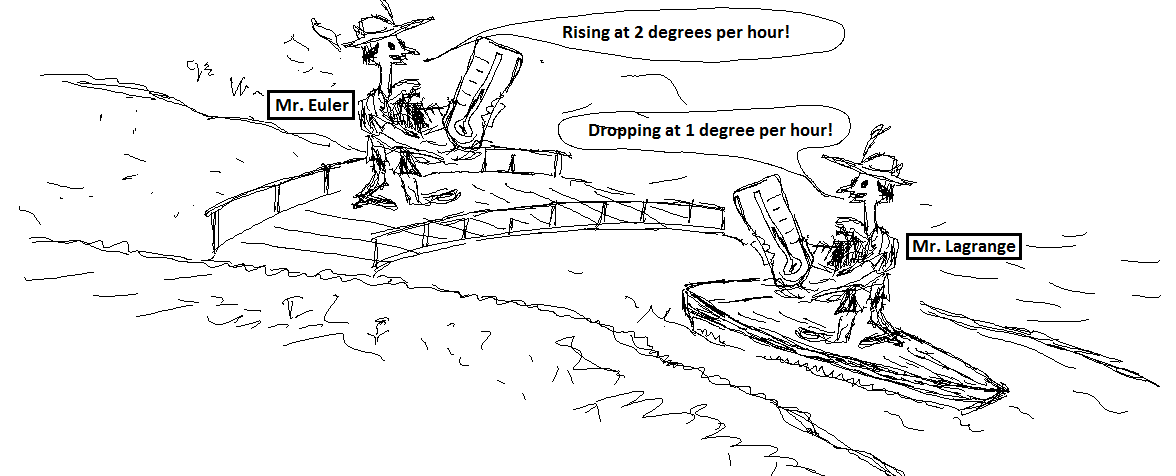
\includegraphics[width=0.6\textwidth]{img/MaterialDerivative.png}
\end{center}

En este curso vamos a adoptar la descripción \textbf{Euleriana}.
    
\end{frame}


%\begin{frame}{Representación del transporte}
%
%\begin{center}
%    
%\begin{tikzpicture}
%\begin{axis}[axis lines = empty]%center, ticks=none, axis on top, axis line style = {thick, black!80}]%[grid=both]
%    \addplot3[surf,fill=white, %shader=faceted interp,
%    samples=10, %point meta rel=per plot,
%    point meta={0}]{0};
%\end{axis}
%    \draw[-latex,ultra thick,blue!90] (2.5,4)--(4.5,4.2) node[above]{$u$};
%    \pause
%\begin{axis}[axis lines = center, ticks=none, axis on top, axis line style = {thick, black!80}]%[grid=both]
%    \addplot3[surf,
%    shader=faceted interp,
%    samples=10,point meta rel=per plot,
%    point meta={sin(deg(x))*sin(deg(y))+0.1*x+0.2*y}   
%    ] {0}; 
%\end{axis}
%\end{tikzpicture}
%\end{center}
%\end{frame}

\begin{frame}{Representación del transporte}

\textbf{Objetivo del curso:} Representar la concentración de un contaminante atmosférico (C) en el espacio y en el tiempo.\\[1em]

Podemos usar el concepto de \textit{función}:
\begin{center}
    \begin{tikzpicture}[scale=0.8,
    >=stealth,
    bullet/.style={ fill=black, circle, minimum width=1pt, inner sep=1pt},
    every fit/.style={ ellipse, draw, inner sep=0pt }
    ]
    \node[bullet] (START) at (0,3){};
    \node[bullet] (END) at (8,3){};
    
    \node[anchor=north] at (START) {(x,y,z,t)};
    \node[anchor=north] at (END)  {c};
 
    \draw (0,2.5) ellipse (1.1cm and 1.7cm);
    \draw (8,2.5) ellipse (1.1cm and 1.7cm);
 
    \pause
    \draw [line width=5pt, blue, shorten <=0.2cm,, shorten >=0.1cm, ->] (START.south) to[out=15, in=165 ] (END);
    \node[blue] at (4,4.1){$c(x,y,z,t)$};

    \end{tikzpicture}
\end{center}
   
   
\end{frame}


 \begin{frame}{Ecuación de transporte}
\pause
Es una \textit{ecuación diferencial}\footnote{Ecuación cuya incógnita es una función} basada en el \textbf{principio de conservación de masa}.\\[2em]
\pause

Describe cómo cambia la concentración  de una especie química (C) en el tiempo para un punto del espacio.\\[2em]
%\item ¿Cómo? descripción \textbf{Euleriana} y \textbf{Lagrangiana}
\pause

Se deduce de analizar todos los procesos que generan un cambio en la concentración en un punto arbitrario del espacio.\\[2em]

%Objetivo:
%$$\boxed{\dfrac{\partial C}{\partial t} }$$
%%- ¿Porqué me interesaría saber esto?\\[1em]
% Si conocemos $C_t$ (condición inicial), y tenemos $\frac{\Delta C}{\Delta t}$ (Ecuación de transporte) entonces podemos predecir como va a ser C para algún tiempo futuro ($C_{t+1}$)\\[1em]
%%-¿Cómo? \\[1em] 
%%- Así:
%\pause
%  $$C_{t+1} = C_{t} + \dfrac{\Delta C}{\Delta t}$$
\end{frame}


\begin{frame}{}
    
\begin{tikzpicture}[remember picture, overlay]
    \node[opacity=1.,inner sep=1pt] (image) at (current page.center) {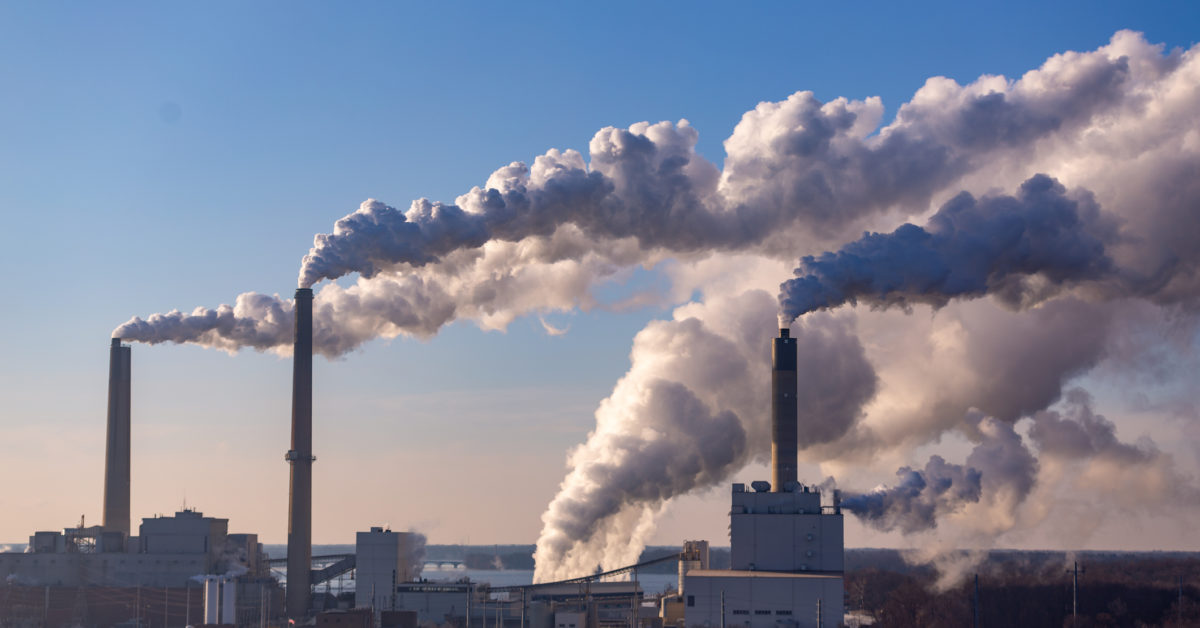
\includegraphics[height=\paperheight, width=1\paperwidth]{img/pollution_plumes.jpg}};
   \begin{scope}[x={(image.south east)},y={(image.north west)}]
        \pause
        \fill[red] (0.22,0.28) circle[radius=2pt] ++(0,0.06) node[anchor=south] {\textbf{Emisión}};
        \pause
        %Adveccion
        \draw[-stealth,ultra thick,blue] (0.4,0.7)--++(0.1,0.15) node[midway,anchor=north]{$\vec{u}$}node[midway,anchor=south]{\textbf{Advección}};
        \pause
        %Mezcla
        \draw[stealth-stealth,ultra thick,black!20!green] (0.6,0.85)--++(0.01,0.5)node[midway,anchor=west]{\textbf{Mezcla}};
        \pause
        %Quimica
        \draw[black!10!yellow] (0.8,0.9) node[anchor=south] {\textbf{Química}};
   \end{scope}
\end{tikzpicture}
\end{frame}
%






%% \begin{frame}{Objetivo}{Encontrar expresión matemática para $\Delta C/\Delta t$}
%%- ¿Cómo hacemos?\\[1em]
%\pause
%\begin{tikzpicture}
%    \node[anchor=south west,inner sep=0] (image) at (0,0) {\includegraphics[width=1\textwidth]{img/spersion-scheme.png}};
%   \begin{scope}[x={(image.south east)},y={(image.north west)}]
%        %\draw[red,help lines,xstep=.1,ystep=.1] (0,0) grid (1,1);
%        %\foreach \x in {0,1,...,9} { \node [anchor=north] at (\x/10,0) {0.\x}; }
%        %\foreach \y in {0,1,...,9} { \node [anchor=east] at (0,\y/10) {0.\y}; }
%        \pause
%        \fill[red] (0.085,0.45) circle[radius=2pt] ++(0,0.06) node[anchor=south] {\textbf{Emisión}};\pause
%        \draw[-stealth,ultra thick,blue] (0.4,0.7)--(0.5,0.7)node[midway,anchor=north]{$\vec{u}$}node[midway,anchor=south]{\textbf{Advección}};\pause
%        \draw[stealth-stealth,ultra thick,black!20!green] (0.3,0.3)--(0.3,0.6)node[midway,anchor=west]{\textbf{Mezcla}};\pause
%        \draw[black!10!yellow] (0.55,0.4) node[anchor=south] {\textbf{Química}};\pause
%   \end{scope}
%\end{tikzpicture}
%
%%\includegraphics[width=1\textwidth]{img/dispersion-scheme.png}
%\pause
%Seleccionamos un volumen infinitesimal arbitrario y analizamos todos los procesos que extraen/incorporan C a dicho volumen. Luego sumamos la contribución de todos los procesos que modifiquen C.
%
%\end{frame}

\section{Emisiones}
\begin{frame}{Emisiones}{Tasa de producción de c}

Representa los procesos que incorporan masa al sistema.
\begin{center}
    \EmisPict
\end{center}

\pause
$$\boxed{\dfrac{\partial c}{\partial t}=E\,}$$

$E$ depende del espacio y el tiempo (donde y cuando es emitido). 

En la pràctica, puede ser medido ó estimado.
%\footnote{Por ejemplo: [E] = kg/s.m2 }
\end{frame}


\section{Reacciones químicas}
 
\begin{frame}{Reacciones químicas}
\begin{center}
\QuimPict
\end{center}
 
 Vamos a considerar los siguientes procesos:
%\begin{columns}[T]
%\column{0.35\textwidth}
\begin{itemize}%[<+->]
\item Química %<1>
\item Fotoquímica %<2>
\item Lavado  %<3>
\item Deposicion seca %<4>
\end{itemize}
 
La probabilidad de ocurrencia de estos fenómenos depende de la cantidad de C presente:
\pause
$$ \dfrac{\partial c}{\partial t} = - \lambda c $$
 
\end{frame}







\section{Advección}
%\pdfliteral direct{2 Tr 0.2 w}
\begin{frame}{Flujo advectivo}{Arrastre por el viento}
\begin{center}
\AdvectPict
\end{center}
\pause
$$
\begin{aligned}
\Delta m =&( {\color{blue} Q_1 c_1}  -   {\color{red} Q_2 c_2} ) \Delta t &\\ \pause
\Delta c\,V =&(A u_1 c_1  -  A u_2 c_2) \Delta t &\\\pause
\Delta c\,\Delta x \Delta y \Delta z  =&( u_1 c_1  -  u_2 c_2)\Delta y\Delta z \Delta t &\\\pause
%\Delta C \Delta x \cancel{\Delta y \Delta z}  =&(u_1 C_1  - u_2 C_2) \cancel{\Delta y \Delta z}  \Delta t &\\\pause
\dfrac{\Delta c}{\Delta t} =& - \dfrac{(u_2 c_2 - u_1 c_1)}{\Delta x}
\end{aligned}
$$
\pause
En el límite $\Delta x\to 0$ , $\Delta t \to 0$:
   $$\boxed{ \dfrac{\partial c} {\partial t}=-\dfrac{\partial (uc)}{\partial x} }$$
   
\end{frame}

\begin{frame}{Intuición}{Advección}
\begin{columns}
\begin{column}{0.5\textwidth}
\begin{tikzpicture}
  \begin{axis} [axis lines=center,ymin=0,ymax=15,xmin=0,xmax=5]
  \draw[-stealth,ultra thick,blue] (2,14)--(3,14)node[anchor=south,midway]{$\vec{u}$};
    \addplot [domain=0:4.7, smooth, thick,red!80] { (x-2)^3 - 5*(x-2) +8};
    %\fill[red] (0.8,12.4) circle[radius=2pt] ++(0,0.1) node[anchor=south] {$p_0$};\pause   
    \fill[red] (2,8) circle[radius=2pt] ++(0,-0.1) node[anchor=north] {$p_1$};%\pause  
    \fill[red] (3.3,3.9) circle[radius=2pt] ++(0,-0.1) node[anchor=north] {$p_2$};%\pause
    \fill[red] (4.5,11) circle[radius=2pt] ++(0,0.1) node[anchor=south] {$p_3$};%\pause   
    
    \addplot [domain=0:5, smooth, thick,dotted,blue!60] { (x-2.3)^3 - 5*(x-2.3) +8};
  \end{axis}
\end{tikzpicture}
\end{column}
\begin{column}{0.5\textwidth}  %%<--- here
    \begin{center}
    \Large 
    $$\begin{aligned}
    \text{  }& - \vec{u} &\quad \dfrac{\partial c}{\partial x}& =&\dfrac{\partial c}{\partial t}\\[1em]\hline
    \text{p1}&\quad(-) &\quad (\square)&\,=\,&\,(\square)\uparrow \\[0.6em]\hline
    \text{p2}&\quad(-) &\quad (\square)&\,=\,&\,(\square)\quad \\       \hline
    \text{p3}&\quad(-) &\quad (\square)&\,=\,&\,(\square)\downarrow \\[0.6em]\hline
    \end{aligned}
    $$ 
    \end{center}
    \vfill
\end{column}
\end{columns}
 
\end{frame}

\section{Mezclado turbulento}
\begin{frame}{}
        \begin{tikzpicture}[remember picture, overlay]
            \node[opacity=1.,inner sep=1pt] at (current page.center)
            {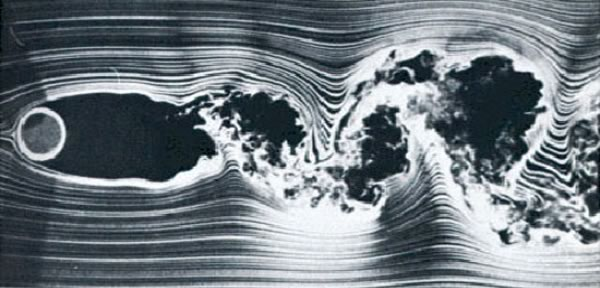
\includegraphics[width=0.98\textwidth]{img/flujo-alrededor-cilindro.jpg}};
        \end{tikzpicture}
 \footnote{tomado de \textit{An album of fluid motion}, de Milton Van Dyke.}
\end{frame}

\begin{frame}{Turbulencia}{Mezclado por turbulencia}

\textit{La turbulencia es parte del flujo no principal que experimenta variaciones abruptas, irregulares, y caóticas.}\\[0.5em]

La turbulencia produce mezclado de las especies químicas en la atmósfera.\\[0.5em]
\pause

 El mezclado debido a la turbulencia tiene naturaleza difusiva, por lo tanto aplica la \alert{Primer ley de Fick:}
 $$\boxed{J=-K\,\dfrac{\partial c }{\partial x} }$$
\pause


El flujo neto de c  (J) debido a la difusión es negativamente proporcional al gradiente de concentraciones.
\end{frame}



\begin{frame}{Mezclado turbulento}

\begin{center}
    \DiffPict
\end{center}

$$
\begin{aligned}
\Delta m   &= ({\color{blue}J_1 A }- {\color{red}J_2 A})\Delta t\\ \pause
\Delta c \Delta x \Delta y \Delta z &= (J_1 - J_2) \Delta y \Delta z\Delta t\\ \pause
\dfrac{\Delta c}{\Delta t} &= \dfrac{J_1 - J_2}{\Delta x}\\ \pause
\dfrac{\Delta c}{\Delta t}&= - \dfrac{(-K_2\frac{\partial c_2}{\partial x}) - (-K_1\frac{\partial c_1}{\partial x})}{\Delta x}\\
\end{aligned}
$$
\pause
En el límite $\Delta x\to 0$ , $\Delta t \to 0$:
\pause
    $$\dfrac{\partial c} {\partial t}=-\dfrac{\partial}{\partial x} - K\dfrac{\partial c}{\partial x}=K\dfrac{\partial^2 c}{\partial x^2}$$
\end{frame}
\begin{frame}{Intuición}{Difusión}
 \begin{columns}
 \begin{column}{0.5\textwidth}
 \begin{tikzpicture}                   
   \begin{axis} [axis lines=center,ymin=0,ymax=15,xmin=0,xmax=5]        
     \addplot [domain=0:4.7, smooth, thick,red!80] { (x-2)^3 - 5*(x-2) +8};
     \fill[red] (0.8,12.4) circle[radius=2pt] ++(0,0.1) node[anchor=south] {$p_1$};%\pause
     \fill[red] (2,8) circle[radius=2pt] ++(0,0.1) node[anchor=south] {$p_2$};%\pause
     \fill[red] (3.3,3.9) circle[radius=2pt] ++(0,-0.1) node[anchor=north] {$p_3$};%\pause
     \addplot [domain=0:5, smooth, thick,dotted,blue!60] {0.7* (x-2)^3 - 5*(x-2)*0.7 +8};          
   \end{axis}                                                                                    
 \end{tikzpicture}            
 \end{column}
 \begin{column}{0.5\textwidth}  %%<--- here
     \begin{center}
     \Large 
     $$
     \begin{aligned}
     \text{  }& K &\quad \dfrac{\partial^2 c}{\partial x^2}& =&\dfrac{\partial c}{\partial t}\\[1em]\hline
     \text{p1}\qquad& (+) &\quad (\square)&\,=\,&\,(\square)\downarrow \\[0.6em]\hline
     \text{p2}\qquad& (+) &\quad (\square)&\,=\,&(\square)\quad \\       \hline
     \text{p3}\qquad& (+) &\quad (\square)&\,=\,&\,(\square)\uparrow \\[0.6em]\hline
     \end{aligned}
     $$ 
    \end{center}
    \vfill
 \end{column}
 \end{columns}
\end{frame}

%\vfill
%\column{0.65\textwidth}

% \only<1> {\begin{block}{Química}
% $X_1 + X_2 \rightarrow X_3 $\\
% $X_1 + X_2 + M \rightarrow X_3 + M $

% $$ \dfrac{\partial [X_{i}]}{\partial t} = S_{i}\omega_r $$

% $$k_{r}[X_1][X_2] \qquad k_{r}[X_1][X_2][M] $$
% \textit{ley de Arrenius}:
% $$k_r (T) = \alpha T^\beta exp(\frac{E_a}{RT}) $$
% \end{block} }

% \only<2> { \begin{block}{Fotoquímica}
% %$$\dfrac{\partial [X_{i}]}{\partial t} = P_{i}- L_{i}[X_{i}] $$
% $AB  + h\nu \rightarrow A + B $
% $$\dfrac{\partial [AB]}{\partial t}= \sigma_{\lambda} I_{\lambda} [AB]$$
% \end{block} }

% \only<3> { \begin{block}{Deposicion húmeda}
%  \textit{scavegging fraction rate} ($\Lambda$)
% $$\Lambda=\alpha P^{\beta}$$
% donde P es la precipitación, y $\alpha$, $\beta$ son parámetros que dependen del contaminante y el mecanismo de remoción.

% \end{block}  }

% \only<4> {\begin{block}{Deposición seca}
%  para la fase gaseosa:
% $$v_{d} =\dfrac{1}{R_a+R_b +R_c}$$
% donde $R_a$ , $R_b$ y $R_c$ son las resistencias aerodinámica, de flujo cuasi-laminar y de superficie respectivamente.
% \textit{ley de Stokes}:
% $$v_d =\dfrac{C\delta g d^{2}}{18\eta}$$
% \end{block}  }
%\end{columns}
%\only<5> {$$\boxed{\dfrac{\partial C}{\partial t}=  \pm R_{Q}\pm R_{FQ}\pm R_{L} \pm R_{D}+... =\sum_{i}^{C}R_{i}} $$}


\section{Ecuación de transporte}
\begin{frame}{Ecuación de transporte}

Finalmente, si sumamos todos los procesos, la ecuación de transporte nos queda:

%    $$\boxed{\dfrac{\partial C}{\partial t}= E - u\dfrac{\partial C}{\partial x}+ K\dfrac{\partial^2C}{\partial x^2} - \lambda C
%}$$
$$
\boxed{
    \dfrac{\partial c}{\partial t}  
    =
    \underbrace{E }_{\text{Emisión}}
    -
    \underbrace{\lambda \,c}_{\text{Química}}
    -
    \underbrace{u \dfrac{\partial c}{\partial x}  }_{\text{Advección}}
    +
    \underbrace{K \dfrac{\partial^2 c}{\partial x^2} }_{\begin{smallmatrix}\text{Mezclado}\\ \text{turbulento} \end{smallmatrix}}
}
$$
% \footnote{
% En 3-dimensiones:
%\begin{equation}
%    \dfrac{\partial C}{\partial t}= E - \nabla \cdot (\vec{v}C) + K\nabla^{2}C \pm \sum_{i=1}^{C} R_{i}
%\end{equation}
%}

\vspace{1.5em}
Para cada situación va a ser necesesario definir los parámetros: $E$, $\lambda$, $u$ y $K$
\end{frame}

 %Ecuacion de transporte (en principio no se va a dar)
   
   %%% Introducción a los modelos gaussianos:
   %\subtitle{Modelos Gaussianos}
 \begin{frame}{}
     \maketitle
 \end{frame}

%\section{Resolución de ecuación de transporte}
\begin{frame}{Resolución de la ecuación de transporte}

    Modelar la química atmosférica consiste en resolver la \alert{ecuación de transporte}:\footnote{$c$: concentración de especie quimica, $v$: velocidad del viento, $K$: coeficiente de turbulencia, $E$: tasa de emisión, $\lambda$: constante de reacción/degradación.}
    
    $$
    \dfrac{\partial c}{\partial t}  
    =
    \underbrace{E }_{\text{Emisión}}
    -
    \underbrace{\lambda \,c}_{\text{Química}}
    -
    \underbrace{u \dfrac{\partial c}{\partial x}  }_{\text{Advección}}
    +
    \underbrace{K \dfrac{\partial^2 c}{\partial x^2} }_{\begin{smallmatrix}\text{Mezclado}\\ \text{turbulento} \end{smallmatrix}}
    $$
    
    Expresa la \textit{conservación de masa} para una especie $c$ transportado por la atmósfera.\\[.5em]

\pause

Hay dos caminos para resolverla:
\begin{columns}
\column{0.5\textwidth}
    \begin{exampleblock}{Analítico}
        \begin{itemize}
            \item Solución exacta. 
            \item Utiliza supuestos y simplificaciones.
            \item Muy rápidos de computar.
        \end{itemize}
    \end{exampleblock}
    
\column{0.5\textwidth}
    \begin{alertblock}{Numérico}
        \begin{itemize}
            \item Solución aproximada.
            \item Sin supuestos ni simplificaciones.
            \item Demandan mucho poder de cálculo.
        \end{itemize}
    \end{alertblock}
\end{columns}
\end{frame}

\section{Solución Analítica a Ecuación de Transporte}
\begin{frame}{Solución Analítica}{Modelos Gaussianos}

Dan la solución a: %\footnote{Desprecia advección en $y$ y $z$}

$$
\dfrac{\partial c}{\partial t} = - u \dfrac{\partial c}{\partial x}+K_x\dfrac{\partial^2 c}{\partial x^2}  
$$

\pause
Cuya solución analítica tiene la forma:\footnote{$\mu= u t$, $\sigma_x=\sqrt{2K_xt}$}

$$c_{(x,t)}=\frac{M}{\sqrt{2\pi } \sigma_{x} } \exp \bigg[ - \frac{1}{2} \frac{ (x-\mu)^2}{\sigma_x^2}  \bigg]$$

\pause
\centering
\begin{center}
\begin{tikzpicture}[baseline=(current bounding box.center),font=\small]
    \begin{axis}[%no markers,
      domain=-3:2, samples=60,
      axis lines*=left, xlabel=$x$, ylabel=$c_{(x)}$,
      height=3cm, width=6cm,
      xtick=\empty, ytick=\empty,
      enlargelimits=false, clip=false, axis on top,
      grid = major
      ]
      \addplot [very thick,color=blue!70,fill=blue!40,text=black!80] {gauss(-1,.5)};%,cyan!50!black,fill=cyan!50!black!20
      \draw [|-|,thick,red!80](-1,0) -- node [midway,anchor=north] {$\sigma$} (-.5,0);
      \draw [dotted,red!80](-1,0) --  (-1,1.) node {$\mu$};
    \end{axis}
\end{tikzpicture}
\end{center}
%\begin{tikzpicture}[baseline=(current bounding box.center)]
%    \begin{axis}[%no markers,
%      domain=-3:5, samples=100,
%      axis lines*=left, xlabel=$x$, ylabel=$c_{(x)}$,
%      height=3cm, width=6cm,
%      xtick=\empty, ytick=\empty,
%      enlargelimits=false,
%      clip=false, axis on top,
%           ylabel near ticks, ylabel shift={4pt},xlabel near ticks, xlabel shift={4pt},
%      ]
%      \addplot [very thick,blue!50,fill=blue!50] {gauss(-1,.5)};
%      \addplot [dashed, very thick,blue!50,fill=blue!50,opacity=0.5] {gauss(2,1)};
%          
%      \draw[|-|,very thick](-1,0) -- node [midway,anchor=north] {\small$\sigma$} (-.5,0);
%      \draw[dotted](-1,0)--(-1,1.) node {\small$\mu$};
%      \draw[-latex,red!75](-1,0.5)--(2,.5) node [midway,anchor=south] {\small$\vec{u}\Delta t$};
%      \draw[dotted](2,0)--(2,1.0) node {\small$\mu + u \Delta t$};
%    
%    \end{axis}
%\end{tikzpicture}

\end{frame}


\begin{frame}{Intuición solución analítica}
    
    Graficar solución analítica:
    
    \begin{center}
    \Large
        \href{https://www.desmos.com/calculator}{https://www.desmos.com/calculator}
    \end{center}
    
    Discusión:
    \begin{itemize}
        \item  Interpretar parámetros ($\mu$ y $\sigma$).
        \item Representa difusión?
        \item Representa advección?
        \item Garantiza conservación de masa?
        \item Incluir término de decaimiento.
    \end{itemize}
    
\end{frame}

\section{Puff Gaussiano}

\begin{frame}{Puff Gaussiano}{Solución \alert{transitoria} }

Resuelve:   
$$ \dfrac{\partial c}{\partial t} = - u \dfrac{\partial c}{\partial x} + K_x\dfrac{\partial^2 c}{\partial x^2} +K_y\dfrac{\partial^2 c}{\partial y^2} +K_z\dfrac{\partial^2 c}{\partial z^2} $$

\pause

Cuya solución es\footnote{$\mu= u t$, $\sigma_{*}=\sqrt{2K_{*}t}$}:
     $$\begin{array}{ll}
     C_{(x,y,z,t)} = & \dfrac{M}{\sqrt{2\pi}^3\sigma_x\sigma_y\sigma_z} \exp \bigg[ - \dfrac{(x-ut)^2}{2\sigma_x^2} \bigg] \exp \bigg[ -\dfrac{y^2}{2\sigma_y^2} \bigg] \exp \bigg[ - \dfrac{z^2}{2\sigma_z^2} \bigg] 
     \end{array}
     $$

\pause
%Here begins the 3D plot
\begin{center}
\begin{tikzpicture}[scale=0.44]
    \begin{axis}[xshift=-4cm,zmax=1]
        \addplot3[surf,samples=30]{1.00*exp(-(y+0.5)^2/2)*exp(-(x+0.5)^2/2)};
    \end{axis}
    \begin{axis}[xshift=4cm,zmax=1.0]
        \addplot3[surf,samples=30]{0.75*exp(-(y-0.5)^2/2)*exp(-(x-0.5)^2/2)};
    \end{axis}
    \begin{axis}[xshift=12cm,zmax=1.0]
        \addplot3[surf,samples=30]{0.40*exp(-(y-1.5)^2/3)*exp(-(x-1.5)^2/3)};
    \end{axis}
\end{tikzpicture}
\end{center}
%Here ends the 3D plot
\end{frame}

%\begin{frame}{Puff Gaussiano}{Supuestos}
%    
%\end{frame}



\section{Pluma Gaussiana}

\begin{frame}{Pluma Gaussiana}{Solución \alert{estacionaria}}

Si planteamos la condición de equilibrio:\footnote{Despreciamos la mezcla turbulenta en $x$ ya que es muy chico comparado con la advección.}
$$
\dfrac{\partial c}{\partial t} =0= - u \dfrac{\partial c}{\partial x}  +K_y\dfrac{\partial^2 c}{\partial y^2} +K_z\dfrac{\partial^2 c}{\partial z^2} $$

Despejando:
$$  \dfrac{\partial c}{\partial x} =  \dfrac{K_{y}}{u} \dfrac{\partial^2 c}{\partial y^2}  +\dfrac{K_{z}}{u} \frac{\partial^2 c}{\partial z^2} $$
\end{frame}

\begin{frame}{Pluma Gaussiana}{Solución \alert{estacionaria}}
 
Resuelve:
$$  \dfrac{\partial c}{\partial x} =  \dfrac{K_{y}}{u} \dfrac{\partial^2 c}{\partial y^2}  +\dfrac{K_{z}}{u} \frac{\partial^2 c}{\partial z^2} $$
 
\pause

Cuya solución es:\footnote{Dado que $t = x/u = cte.$, entonces:  $\sigma_i=\sqrt{2K_i t}=\sqrt{2 K_i x/u}$.}

$$
c_{(x,y,z)} = \dfrac{Q}{u\sqrt{2\pi}^2\sigma_y\sigma_z} \exp \bigg[ -\dfrac{y^2}{2\sigma_y^2} \bigg] \exp \bigg[ - \dfrac{z^2}{2\sigma_z^2} \bigg] 
$$
     
\pause
%Here begins the 3D plot
\begin{center}
\begin{tikzpicture}[scale=0.45]
    \begin{axis}[xshift= -5cm,domain=0.01:15,
        y domain=-10:10]%,xmin=0.01,ymin=-10,ymax=10]%,zmax=1]
        \addplot3[contour filled={number=13}, samples=60]{1.00/sqrt(x)*exp(-(y)^2/x)};
    \end{axis}
    \begin{axis}[xshift= 5cm,domain=0.01:15,
        y domain=-10:10,view={0}{90}]%,xmin=0.01,ymin=-10,ymax=10]%,zmax=1]
        \addplot3[contour filled={number=13}, samples=90]{1.00/sqrt(x)*exp(-(y)^2/x)};
    \end{axis}
\end{tikzpicture}
\end{center}
%Here ends the 3D plot
\end{frame}

%\begin{frame}{Pluma Gaussiana}{Supuestos}
%    
%\end{frame}

\begin{frame}{Comparación Pluma Gaussiana con experimento de Richardson}

\begin{center}
\begin{tikzpicture}[scale=0.45]
 \node[opacity=1.,inner sep=1pt] (image) at (current page.center){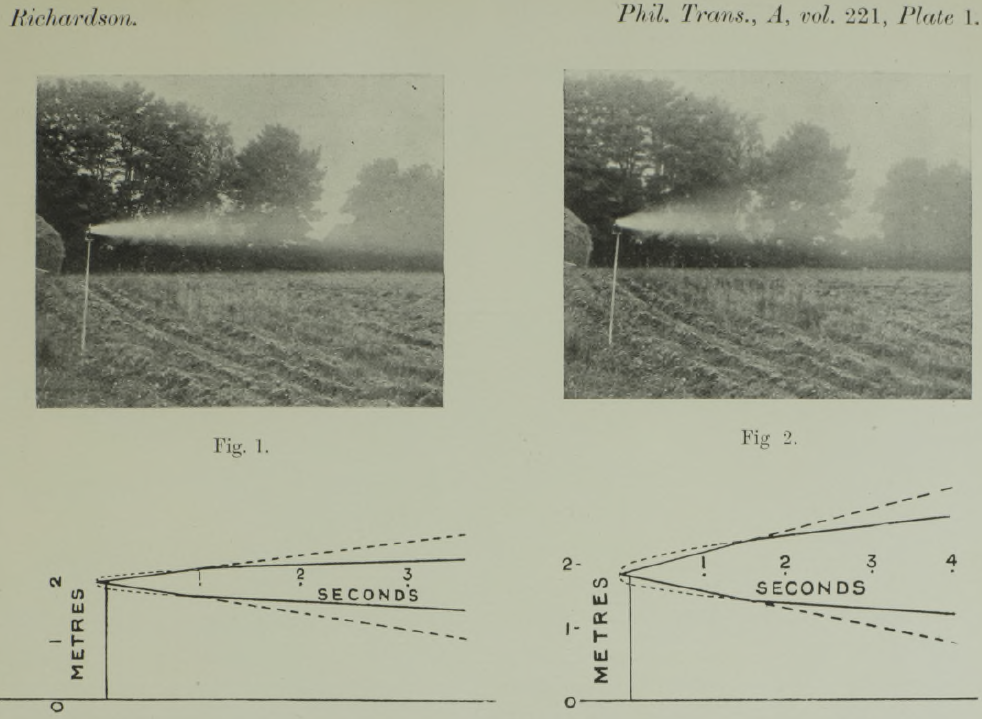
\includegraphics[width=0.65\textwidth]{img/richardsonPlumas-1921.png}};
\end{tikzpicture}
\end{center}

\end{frame}
%
%
%\section{Modificacciones a modelo Gaussiano}
%
%%\begin{frame}{Descomposición de operadores}
%%    
%%    
%%    $$c_{(x,y,z)} = \frac{Q}{u}\, \Phi_x \Phi_y \Phi_z  $$
%%    
%%    donde:
%%    $$\Phi_x = 1 $$
%%    $$\Phi_y = \dfrac{1}{\sqrt{2\pi} \sigma_y}\exp{\bigg( \dfrac{y^2}{2\sigma_y^2}\bigg)}$$
%%    $$\Phi_z = \dfrac{1}{\sqrt{2\pi} \sigma_z}\exp{\bigg( \dfrac{z^2}{2\sigma_z^2}\bigg)}$$
%%    
%%\end{frame}
%
%
%\begin{frame}[t]{Altura de la fuente}
%    \centering
%\begin{tikzpicture}[scale=1.3]
%     \clip(-4,-1) rectangle (4,2);
%%axis:
%\ejesXZ{-5}{0}{0.45}
%%piso
%\piso{-4}{4.5}{0}
%\chimenea{-3.1}{0}{0.2}{1.2}
%%\draw[fill=black!60](#1,#2) rectangle ++(#3,#4);
%%\node(chim1)[fill=black!60,minimum height=1.25cm] at (-3.1,0.6){};
%%\fill[red!20,opacity=0.5] (chim1.north) -- (4,2) -- (4,-1) -- (chim1.north);
%\fill[red!20,opacity=0.5] (-3.1,1.2) -- (4,2) -- (4,-1) -- (-3.1,1.2);
% 
%\draw[| latex-latex] (-3.2, 1.2)--(-3.2,0) node[midway, anchor=east]{$H$};
% 
%\end{tikzpicture}
% 
%     $$\begin{array}{ll}
%     C_{(x)} = & \dfrac{Q}{u\sqrt{2\pi}^2\sigma_y\sigma_z} \exp \bigg[ -\dfrac{y^2}{2\sigma_y^2} \bigg] \exp \bigg[ - \dfrac{(z\alert{-H})^2}{2\sigma_z^2} \bigg] 
%     \end{array}
%     $$
% 
%\end{frame}
% \begin{frame}{Altura efectiva}{Plume Rise}
% 
%\begin{center}
%\begin{tikzpicture}[scale=1.3]
%     \clip(-4,-0.5) rectangle (4,2);
% \ejesXZ{-5}{0}{0.45}
% \piso{-4}{4.5}{0}
% \chimenea{-3.1}{0}{0.2}{1.2}
%  %pluma real
% \fill[red!20,opacity=0.5] (-3.1,1.75) -- (4,2) -- (4,0.5) -- (-3.1,1.75);
%  \draw[| latex-latex] (-3.2, 1.2)--(-3.2,0) node[midway, anchor=east]{$H$};
%  \draw[| latex-latex] (-3.2, 1.2)--(-3.2,1.75) node[midway, anchor=east]{$\Delta h$};
%  \end{tikzpicture}
% \end{center}  
%
%Elevación por empuje térmico y e impulso en la fuente.
%  
%    $$
%    C_{(x)} = \dfrac{Q}{u\sqrt{2\pi}^2\sigma_y\sigma_z} \exp \bigg[ -\dfrac{y^2}{2\sigma_y^2} \bigg] \exp \bigg[ - \dfrac{(z-H - \alert{\Delta h})^2}{2\sigma_z^2} \bigg] 
%    $$
% 
% \end{frame}
% 
% 
% 
% 
%\begin{frame}[t]{Edificios y obstaculos}{Downwash}
%
%\begin{center}
%\begin{tikzpicture}[scale=1.3]
%     \clip(-4,-0.5) rectangle (4,2);
%%axis:
%\ejesXZ{-5}{0}{0.45}
%%piso
%\piso{-4}{4.5}{0}
%%pluma real
%\chimenea{-3.1}{0}{0.2}{1.2}
%\fill[red!20,opacity=0.5] (-3,1.2) --(0,1.4)to[out=0,in=182] (4,1.2) -- (4,0) to[out=180, in=-5] (0,1) -- (-3,1.2);
% 
%\draw[| latex-latex] (-3.2, 1.2)--(-3.2,0) node[midway, anchor=east]{$H$};
% 
%\draw[building](0,0) rectangle (0.5,0.8);
% 
%%remolinos
%\draw [>=stealth,->,blue!80] (0.7,0.1) arc (280:0:.1cm) -- +(283:0.05cm);
%\draw [>=stealth,->,blue!80] (0.7,0.3) arc (280:0:.1cm) -- +(283:0.05cm);
%\draw [>=stealth,->,blue!80] (0.7,0.6) arc (280:0:.1cm) -- +(283:0.05cm);
%\draw [>=stealth,->,blue!80] (1.0,0.2) arc (280:0:.1cm) -- +(283:0.05cm);
%\draw [>=stealth,->,blue!80] (1.0,0.5) arc (280:0:.1cm) -- +(283:0.05cm);
%\draw [>=stealth,->,blue!80] (1.3,0.4) arc (280:0:.1cm) -- +(283:0.05cm);
%\draw [>=stealth,->,blue!80] (1.3,0.1) arc (280:0:.1cm) -- +(283:0.05cm);
%\draw [>=stealth,->,blue!80] (1.6,0.2) arc (280:0:.1cm) -- +(283:0.05cm);
%\draw [>=stealth,->,blue!80] (1.9,0.1) arc (280:0:.1cm) -- +(283:0.05cm);
% 
%\end{tikzpicture}
%\end{center} 
% 
% Deflección por sombra turbulenta generada por edificios y obstaculos:
%    $$
%    C_{(x)} = \dfrac{Q}{u\sqrt{2\pi}^2\sigma_y\sigma_z} \exp \bigg[ -\dfrac{y^2}{2\sigma_y^2} \bigg] \exp \bigg[ - \dfrac{(z-H - \alert{\Delta h})^2}{2\sigma_z^2} \bigg] 
%    $$
%\end{frame}
%
%
%\begin{frame}[t]{Terreno (plano)}{Reflexión}
%    \centering
%\begin{tikzpicture}%[scale=1.3]
%    \clip(-4,-2.0) rectangle (4,2);
%%axis:
%\ejesXZ{-5}{0}{0.45}
%%piso
%\piso{-4}{4.5}{0}
%\node(chim1)[fill=black!60,minimum height=1.25cm] at (-3,0.6){};
%\node(chim2)[fill=black!60,minimum height=1.25cm,opacity=0.5] at (-3,-0.6){};
%
%\fill[red!20,opacity=0.5] (chim1.north) -- (4,2) -- (4,-1) -- (chim1.north);
%\fill[blue!20, opacity=0.3, pattern=north east lines] (chim2.south) -- (4,-2) -- (4,1) -- (chim2.south);
%
%\fill[pattern=north east lines,pattern color=red] (0.8,0) -- (4,0) -- (4,1) --(0.8,0);
%
%\draw[| latex-latex] (-3.2, 1.2)--(-3.2,0) node[midway, anchor=east]{$H$};
%\draw[| latex-latex,opacity=0.5] (-3.2,-1.2)--(-3.2,0) node[midway, anchor=east]{$-H$};
%
%\end{tikzpicture}
% 
%     $$\begin{array}{ll}
%     C_{(x)} = & \dfrac{Q}{u\sqrt{2\pi}^2\sigma_y\sigma_z} \exp \bigg[ -\dfrac{y^2}{2\sigma_y^2} \bigg] \bigg(\exp \bigg[ - \dfrac{(z-H)^2}{2\sigma_z^2} \bigg] \alert{+ \exp \bigg[ - \dfrac{(z+H)^2}{2\sigma_z^2} \bigg]}\bigg)
%     \end{array}
%     $$
% 
%\end{frame}
%
%
%
%
%\begin{frame}[t]{Terreno complejo}{}
% 
%\centering
%\begin{tikzpicture}[scale=1.3]
%\ejesXZ{-5}{0}{0.45}
%\piso{-4}{4.5}{0}
%\chimenea{-3.1}{0}{0.2}{1.2}
%%pluma real
%\fill[red!20,opacity=0.5] (-3,1.2) -- (4,2.2) -- (4,0.4) -- (-3,1.2);
%%mountain
%\draw[ latex-latex] (-3.2, 1.2)--(-3.2,0) node[midway, anchor=east]{$H$};
%
%     \node[brown] at (0.5,0.8) {\textbullet};
%     \fill[fill=blue] (0.5,1.1) circle[radius=2pt] node[anchor=south west]{$r_1$};
%     \fill[fill=red ] (0.5,0.3) circle[radius=2pt] node[anchor=south west]{$r_2$};
%     
%     \draw[latex-latex] (1.0,0.0)--(1.0,0.8)node[midway,anchor=west]{$z_{t}$}; 
%     \draw[latex-latex] (0.5,0.8)--(0.5,1.1)node[midway,anchor=west]{$z_{p}$}; 
%     \draw[latex-latex] (0.5,0.0)--(0.5,0.3)node[midway,anchor=west]{$z_{p}$}; 
%     \draw[latex-latex] (1.5,0.0)--(1.5,1.1)node[midway,anchor=west]{$z_{r}$};
%     
%     \draw[orange!70, dashed] (-3,0.85)--(4,0.85) node[anchor=west]{$H_c$};
%   \draw[|-|, green] (4.5,0.85)--(4.5,2.2) node[midway, anchor=west]{$M_a$};
%   \draw[|-|, green] (4.5,0.85)--(4.5,0.5) node[midway, anchor=west]{$M_b$};
%   \draw[clip]
%    decorate [decoration={random steps,segment length=3pt,amplitude=1pt}]%
%    {(-1,0) --(0,0.3)-- (0.5,0.8) -- (1,1.5)--(2,2) --(3.0,2.5)-- (3.5,2.3) -- (4,0)}-- (0,0) -- (-1,0);
%    \fill[rock](-1,0) rectangle (4,4);
%        
%\end{tikzpicture}
%
%Se calculan dos plumas, una ignorando el terreno y otra siguiendo el terreno:
%
%$$ C_{tot} = f {\color{blue} C_{ref} } + (1-f) {\color{red}C_{terr.} } $$
%
%El resultado es una ponderación de estas dos determinadas por el factor $f$.
%
%
%\footnote{donde $f=0.5 + 0.5 \varphi_p $ y $\varphi_p= M_b / M_a\,M_b$. $M_a$ Masa sobre $H_c$ y $M_b$ masa por debajo de $H_c$. $h_c$: hill slope scale. $H_c$: critical dividing streamline}
%
%\end{frame}
%
%
%
%
%\begin{frame}{Coeficientes turbulentos}{Estabilidad}
%
%La estabilidad da idea de la libertad que tienen las maasas de aire para moverse verticalmente.
%
%\begin{center}
%\begin{tikzpicture}[scale=0.6]
%
%\begin{scope}[yshift=3cm]
%\ejesXZ{-5}{0}{0.45}
%\piso{-4}{4.5}{0}
%\chimenea{-3.1}{0}{0.2}{1.2}
% %pluma real
%\fill[red!20,opacity=0.5] (-3,1.2) -- (4,2.5) -- (4,0) -- (-3,1.2);
%\node[] at (6,1.2){Inestable};
%\end{scope}
%
%\begin{scope}[yshift=0cm]
%\ejesXZ{-5}{0}{0.45}
%\piso{-4}{4.5}{0}
%\chimenea{-3.1}{0}{0.2}{1.2}
% %pluma real
%\fill[red!20,opacity=0.5] (-3,1.2) -- (4,2) -- (4,0.5) -- (-3,1.2);
%\node[] at (6,1.2){Neutro};
%\end{scope}
%
%\begin{scope}[yshift=-3cm]
%\ejesXZ{-5}{0}{0.45}
%\piso{-4}{4.5}{0}
%\chimenea{-3.1}{0}{0.2}{1.2}
% %pluma real
%\fill[red!20,opacity=0.5] (-3,1.2) -- (4,1.5) -- (4,1.0) -- (-3,1.2);
%\node[] at (6,1.2){Estable};
%\end{scope}
%
%\end{tikzpicture}
%\end{center}
%
%\end{frame}
% 
%\begin{frame}{Coeficientes turbulentos}{Parametrizaciones basadas en clases de estabilidad}
%La clasificación mas usada para determinar la estabilidad atmosférica es la desarrollada por Pasquill (1961) y Gifford (1961). Ellos definieron 6 clases (A-F)\footnote{donde A: muy inestable, B: moderadamente estable, C: levemente estable, D neutral, E levemente estable, F: estable.}
% 
%\begin{table}[]
%    \centering
%\begin{tabular}{| c | c c c | c c |}
%\hline
%& \multicolumn{3}{c|}{Día} & \multicolumn{2}{c|}{Noche} \\
%& \multicolumn{3}{c|}{Radiación solar} & \multicolumn{2}{c|}{Nubosidad} \\
%$u (m/s)$ & Fuerte & Media & Débil & Nublado ($> 4/8$) & Despejado ($<3/8$) \\ \hline
%<2  & A   & A-B  & B & E & F \\ 
%2-3 & A-B & B    & C & E & F \\ 
%3-5 & B   & B-C  & C & D & E \\ 
%5-6 & C   & C-D  & D & D & D \\ 
%>6  & C   & D    & D & D & D \\ \hline
%\end{tabular}
%    \caption{Clases de Estabilidad}
%    \label{tab:my_label}
%\end{table}
%\end{frame}
%
% 
% 
% \begin{frame}{Coeficientes turbulentos}{Parametrizaciones basadas en clases de estabilidad}
%  
% Briggs (1973), propuso formulas empiricas para el calculo de los $\sigma$:
%  
% $$
% \sigma_y =\dfrac{a x}{(1+bx)^c}
% \qquad
% \sigma_z =\dfrac{d x}{(1+ex)^f}
% $$
%  
% Los coeficientes (a,b,c,d,e,f) están tabulados y dependen de la clase de estabilidad:
%  
%{\tiny
% \begin{columns}[t]
%
% 
% \column{0.5\textwidth}
% \begin{table}
%     \centering
% \begin{tabular}{| c | c c  c | c c c |}
% \hline
% C.E&    a &    b   &    c &     d &   e    & f  \\\hline
%  A & 0.22 & 0.0001 &  0.5 & 0.2   & 0      & —  \\     
%  B & 0.16 & 0.0001 &  0.5 & 0.12  & 0      & —  \\
%  C & 0.11 & 0.0001 &  0.5 & 0.08  & 0.0002 & 0.5\\
%  D & 0.08 & 0.0001 &  0.5 & 0.06  & 0.0015 & 0.5\\
%  E & 0.06 & 0.0001 &  0.5 & 0.03  & 0.0003 & 1  \\
%  F & 0.04 & 0.0001 &  0.5 & 0.016 & 0.0003 & 1  \\ \hline
% \end{tabular}
%     \caption{Rural}
% \end{table}
%  
% \column{0.5\textwidth}
% 
% \begin{table}
%     \centering
% \begin{tabular}{| c | c c  c | c c c |}
% \hline
% C.E& a & b & c & d & e & f  \\\hline
% A   & 0.32 & 0.0004 & 0.5 & 0.24  & 0.0001  & -0.5 \\
% B   & 0.32 & 0.0004 & 0.5 & 0.24  & 0.0001  & -0.5 \\
% C   & 0.22 & 0.0004 & 0.5 & 0.2   & 0       & —    \\
% D   & 0.16 & 0.0004 & 0.5 & 0.14  & 0.0003  & 0.5  \\
% E   & 0.11 & 0.0004 & 0.5 & 0.08  & 0.0015  & 0.5  \\ 
% F   & 0.11 & 0.0004 & 0.5 & 0.08  & 0.0015  & 0.5  \\ \hline
% \end{tabular}
%     \caption{Urbano}
% \end{table}
% \end{columns}
% } %(tiny)
% \end{frame}
%  
% \begin{frame}{Coeficientes turbulentos}{Modificadores temporales}
%  
% Los coeficientes de Briggs fueron generados con observaciones de promedios de 10 minutos. Para otros promedios temporales se usa:
% 
% $$ \sigma_{y,2}= \sigma_{y,1} \bigg( \dfrac{t_2}{t_1}\bigg)^p$$
% 
% \end{frame}
%  
% \begin{frame}{Coeficientes turbulentos}{Parametrizaciones continuas}
%  
%  Basadas en el estudio de la turbulencia:
%  
% $$ \sigma_y = \sigma_v \, \dfrac{x}{u} f_y \qquad \sigma_z = \sigma_w \, \dfrac{x}{u} f_z$$
%  
%  donde $\sigma_v$ y $\sigma_w$ son los desvíos estándar de la velocidad del viento en la componente $y$ y $z$ respectivamente.
%  
% \end{frame}
% 
% \begin{frame}{Capa límite}{Inversiones Térmicas}
%  
% \begin{center}
% \begin{tikzpicture}
% \ejesXZ{-5}{0}{0.45}
% \piso{-4}{4.5}{0}
% \chimenea{-3.1}{0}{0.2}{1.2}
% %pluma real
% \fill[red!20,opacity=0.5] (-3,1.2)--(4,2)--(4,-1)--(-3,1.2);
% \draw[| latex-latex] (-3.2, 1.2)--(-3.2,0) node[midway, anchor=east]{$H$};
%  
%  %pluma espejada
%  \begin{scope}[yscale=-1,xscale=1,yshift=-3cm]
%    \chimenea{-3.1}{0}{0.2}{1.2}
%    \fill[black!30, opacity=0.3, pattern=north east lines] (-3,1.2)--(4,2)--(4,-1)--(-3,1.2);
%    %\fill[black!30, opacity=0.3, pattern=north east lines] (chim3.south) -- (4,2) -- (4,-1) -- (chim3.south);
%    \draw[| latex-latex,black!30] (-3.2, 1.2)--(-3.2,0) node[midway, anchor=east]{$-H$};
% \end{scope}
%  
%  \draw[-latex,thick,green!80!black](4,0)--(4,1.5)node[midway,anchor=west]{$Z_{ic}   $};
%  \draw[-,dashed,very thick,blue!30](-4,1.5)--(4,1.5);
%  %diferencia
% %\fill[pattern=north east lines,pattern color=red] (0.8,0) -- (4,0) -- (4,1) --(0.8,0);
% \end{tikzpicture}
%      
%\end{center}
%
%Se resuelve de la misma forma que la reflexión en el suelo.
%
%\end{frame}
% 
% 
% \begin{frame}{Química y Deposición}
%     
%     Generalmente se aproximan con la ecuación de decaimiento exponencial de primer orden:\footnote{$\phi_x=\dfrac{1}{\sqrt{2\,\pi} \exp\bigg\[ -\dfrac{1}{}\bigg]}$}
%     
%     $$ 
%     C_{(x,y,z)} = \dfrac{Q}{u} \phi_y \phi_z \,\alert{\exp \bigg[ -\lambda \frac{x}{u}  \bigg] }
%     $$
%     
%     
%     
%     
% \end{frame}
%  
%
%\begin{frame}{Terreno Urbano/Industrial}
%    
%Un ambiente urbano/industrial se diferencia de uno rural en:
%\begin{itemize}
%    \item Rugosidad (por obstaculos) 
%    \item Balance radiativo (diferencias en reflectividad, y evaporaciòn)
%    \item Turbulencia afectada por ostaculos (entre obstaculos y sobre ellos)
%    \item Perfil de velocidad de vientos (el perfil calculado por teoria de similitud no funciona a alturas de 1-2 alturas de los obstaculos, es decir 10-20 $z0$).
%\end{itemize}
%\end{frame}
%   %Introduccion a los modelos de calidad del aire
   %\section{Modificacciones a modelo Gaussiano}

%\begin{frame}{Descomposición de operadores}
%    
%    
%    $$c_{(x,y,z)} = \frac{Q}{u}\, \Phi_x \Phi_y \Phi_z  $$
%    
%    donde:
%    $$\Phi_x = 1 $$
%    $$\Phi_y = \dfrac{1}{\sqrt{2\pi} \sigma_y}\exp{\bigg( \dfrac{y^2}{2\sigma_y^2}\bigg)}$$
%    $$\Phi_z = \dfrac{1}{\sqrt{2\pi} \sigma_z}\exp{\bigg( \dfrac{z^2}{2\sigma_z^2}\bigg)}$$
%    
%\end{frame}


\begin{frame}[t]{Altura de la fuente}
    \centering
\begin{tikzpicture}[scale=1.3]
     \clip(-4,-1) rectangle (4,2);
%axis:
\ejesXZ{-5}{0}{0.45}
%piso
\piso{-4}{4.5}{0}
\chimenea{-3.1}{0}{0.2}{1.2}
%\draw[fill=black!60](#1,#2) rectangle ++(#3,#4);
%\node(chim1)[fill=black!60,minimum height=1.25cm] at (-3.1,0.6){};
%\fill[red!20,opacity=0.5] (chim1.north) -- (4,2) -- (4,-1) -- (chim1.north);
\fill[red!20,opacity=0.5] (-3.1,1.2) -- (4,2) -- (4,-1) -- (-3.1,1.2);
 
\draw[| latex-latex] (-3.2, 1.2)--(-3.2,0) node[midway, anchor=east]{$H$};
 
\end{tikzpicture}
 
     $$\begin{array}{ll}
     C_{(x)} = & \dfrac{Q}{u\sqrt{2\pi}^2\sigma_y\sigma_z} \exp \bigg[ -\dfrac{y^2}{2\sigma_y^2} \bigg] \exp \bigg[ - \dfrac{(z\alert{-H})^2}{2\sigma_z^2} \bigg] 
     \end{array}
     $$
 
\end{frame}
 \begin{frame}{Altura efectiva}{Plume Rise}
 
\begin{center}
\begin{tikzpicture}[scale=1.3]
     \clip(-4,-0.5) rectangle (4,2);
 \ejesXZ{-5}{0}{0.45}
 \piso{-4}{4.5}{0}
 \chimenea{-3.1}{0}{0.2}{1.2}
  %pluma real
 \fill[red!20,opacity=0.5] (-3.1,1.75) -- (4,2) -- (4,0.5) -- (-3.1,1.75);
  \draw[| latex-latex] (-3.2, 1.2)--(-3.2,0) node[midway, anchor=east]{$H$};
  \draw[| latex-latex] (-3.2, 1.2)--(-3.2,1.75) node[midway, anchor=east]{$\Delta h$};
  \end{tikzpicture}
 \end{center}  

Elevación por empuje térmico y e impulso en la fuente.
  
    $$
    C_{(x)} = \dfrac{Q}{u\sqrt{2\pi}^2\sigma_y\sigma_z} \exp \bigg[ -\dfrac{y^2}{2\sigma_y^2} \bigg] \exp \bigg[ - \dfrac{(z-H - \alert{\Delta h})^2}{2\sigma_z^2} \bigg] 
    $$
 
 \end{frame}
 
 
 
 
\begin{frame}[t]{Edificios y obstaculos}{Downwash}

\begin{center}
\begin{tikzpicture}[scale=1.3]
     \clip(-4,-0.5) rectangle (4,2);
%axis:
\ejesXZ{-5}{0}{0.45}
%piso
\piso{-4}{4.5}{0}
%pluma real
\chimenea{-3.1}{0}{0.2}{1.2}
\fill[red!20,opacity=0.5] (-3,1.2) --(0,1.4)to[out=0,in=182] (4,1.2) -- (4,0) to[out=180, in=-5] (0,1) -- (-3,1.2);
 
\draw[| latex-latex] (-3.2, 1.2)--(-3.2,0) node[midway, anchor=east]{$H$};
 
\draw[building](0,0) rectangle (0.5,0.8);
 
%remolinos
\draw [>=stealth,->,blue!80] (0.7,0.1) arc (280:0:.1cm) -- +(283:0.05cm);
\draw [>=stealth,->,blue!80] (0.7,0.3) arc (280:0:.1cm) -- +(283:0.05cm);
\draw [>=stealth,->,blue!80] (0.7,0.6) arc (280:0:.1cm) -- +(283:0.05cm);
\draw [>=stealth,->,blue!80] (1.0,0.2) arc (280:0:.1cm) -- +(283:0.05cm);
\draw [>=stealth,->,blue!80] (1.0,0.5) arc (280:0:.1cm) -- +(283:0.05cm);
\draw [>=stealth,->,blue!80] (1.3,0.4) arc (280:0:.1cm) -- +(283:0.05cm);
\draw [>=stealth,->,blue!80] (1.3,0.1) arc (280:0:.1cm) -- +(283:0.05cm);
\draw [>=stealth,->,blue!80] (1.6,0.2) arc (280:0:.1cm) -- +(283:0.05cm);
\draw [>=stealth,->,blue!80] (1.9,0.1) arc (280:0:.1cm) -- +(283:0.05cm);
 
\end{tikzpicture}
\end{center} 
 
 Deflección por sombra turbulenta generada por edificios y obstaculos:
    $$
    C_{(x)} = \dfrac{Q}{u\sqrt{2\pi}^2\sigma_y\sigma_z} \exp \bigg[ -\dfrac{y^2}{2\sigma_y^2} \bigg] \exp \bigg[ - \dfrac{(z-H - \alert{\Delta h})^2}{2\sigma_z^2} \bigg] 
    $$
\end{frame}


\begin{frame}[t]{Terreno (plano)}{Reflexión}
    \centering
\begin{tikzpicture}%[scale=1.3]
    \clip(-4,-2.0) rectangle (4,2);
%axis:
\ejesXZ{-5}{0}{0.45}
%piso
\piso{-4}{4.5}{0}
\node(chim1)[fill=black!60,minimum height=1.25cm] at (-3,0.6){};
\node(chim2)[fill=black!60,minimum height=1.25cm,opacity=0.5] at (-3,-0.6){};

\fill[red!20,opacity=0.5] (chim1.north) -- (4,2) -- (4,-1) -- (chim1.north);
\fill[blue!20, opacity=0.3, pattern=north east lines] (chim2.south) -- (4,-2) -- (4,1) -- (chim2.south);

\fill[pattern=north east lines,pattern color=red] (0.8,0) -- (4,0) -- (4,1) --(0.8,0);

\draw[| latex-latex] (-3.2, 1.2)--(-3.2,0) node[midway, anchor=east]{$H$};
\draw[| latex-latex,opacity=0.5] (-3.2,-1.2)--(-3.2,0) node[midway, anchor=east]{$-H$};

\end{tikzpicture}
 
     $$\begin{array}{ll}
     C_{(x)} = & \dfrac{Q}{u\sqrt{2\pi}^2\sigma_y\sigma_z} \exp \bigg[ -\dfrac{y^2}{2\sigma_y^2} \bigg] \bigg(\exp \bigg[ - \dfrac{(z-H)^2}{2\sigma_z^2} \bigg] \alert{+ \exp \bigg[ - \dfrac{(z+H)^2}{2\sigma_z^2} \bigg]}\bigg)
     \end{array}
     $$
 
\end{frame}




\begin{frame}[t]{Terreno complejo}{}
 
\centering
\begin{tikzpicture}[scale=1.3]
\ejesXZ{-5}{0}{0.45}
\piso{-4}{4.5}{0}
\chimenea{-3.1}{0}{0.2}{1.2}
%pluma real
\fill[red!20,opacity=0.5] (-3,1.2) -- (4,2.2) -- (4,0.4) -- (-3,1.2);
%mountain
\draw[ latex-latex] (-3.2, 1.2)--(-3.2,0) node[midway, anchor=east]{$H$};

     \node[brown] at (0.5,0.8) {\textbullet};
     \fill[fill=blue] (0.5,1.1) circle[radius=2pt] node[anchor=south west]{$r_1$};
     \fill[fill=red ] (0.5,0.3) circle[radius=2pt] node[anchor=south west]{$r_2$};
     
     \draw[latex-latex] (1.0,0.0)--(1.0,0.8)node[midway,anchor=west]{$z_{t}$}; 
     \draw[latex-latex] (0.5,0.8)--(0.5,1.1)node[midway,anchor=west]{$z_{p}$}; 
     \draw[latex-latex] (0.5,0.0)--(0.5,0.3)node[midway,anchor=west]{$z_{p}$}; 
     \draw[latex-latex] (1.5,0.0)--(1.5,1.1)node[midway,anchor=west]{$z_{r}$};
     
     \draw[orange!70, dashed] (-3,0.85)--(4,0.85) node[anchor=west]{$H_c$};
   \draw[|-|, green] (4.5,0.85)--(4.5,2.2) node[midway, anchor=west]{$M_a$};
   \draw[|-|, green] (4.5,0.85)--(4.5,0.5) node[midway, anchor=west]{$M_b$};
   \draw[clip]
    decorate [decoration={random steps,segment length=3pt,amplitude=1pt}]%
    {(-1,0) --(0,0.3)-- (0.5,0.8) -- (1,1.5)--(2,2) --(3.0,2.5)-- (3.5,2.3) -- (4,0)}-- (0,0) -- (-1,0);
    \fill[rock](-1,0) rectangle (4,4);
        
\end{tikzpicture}

Se calculan dos plumas, una ignorando el terreno y otra siguiendo el terreno:

$$ C_{tot} = f {\color{blue} C_{ref} } + (1-f) {\color{red}C_{terr.} } $$

El resultado es una ponderación de estas dos determinadas por el factor $f$.


\footnote{donde $f=0.5 + 0.5 \varphi_p $ y $\varphi_p= M_b / M_a\,M_b$. $M_a$ Masa sobre $H_c$ y $M_b$ masa por debajo de $H_c$. $h_c$: hill slope scale. $H_c$: critical dividing streamline}

\end{frame}




\begin{frame}{Coeficientes turbulentos}{Estabilidad}

La estabilidad da idea de la libertad que tienen las maasas de aire para moverse verticalmente.

\begin{center}
\begin{tikzpicture}[scale=0.6]

\begin{scope}[yshift=3cm]
\ejesXZ{-5}{0}{0.45}
\piso{-4}{4.5}{0}
\chimenea{-3.1}{0}{0.2}{1.2}
 %pluma real
\fill[red!20,opacity=0.5] (-3,1.2) -- (4,2.5) -- (4,0) -- (-3,1.2);
\node[] at (6,1.2){Inestable};
\end{scope}

\begin{scope}[yshift=0cm]
\ejesXZ{-5}{0}{0.45}
\piso{-4}{4.5}{0}
\chimenea{-3.1}{0}{0.2}{1.2}
 %pluma real
\fill[red!20,opacity=0.5] (-3,1.2) -- (4,2) -- (4,0.5) -- (-3,1.2);
\node[] at (6,1.2){Neutro};
\end{scope}

\begin{scope}[yshift=-3cm]
\ejesXZ{-5}{0}{0.45}
\piso{-4}{4.5}{0}
\chimenea{-3.1}{0}{0.2}{1.2}
 %pluma real
\fill[red!20,opacity=0.5] (-3,1.2) -- (4,1.5) -- (4,1.0) -- (-3,1.2);
\node[] at (6,1.2){Estable};
\end{scope}

\end{tikzpicture}
\end{center}

\end{frame}
 
\begin{frame}{Coeficientes turbulentos}{Parametrizaciones basadas en clases de estabilidad}
La clasificación mas usada para determinar la estabilidad atmosférica es la desarrollada por Pasquill (1961) y Gifford (1961). Ellos definieron 6 clases (A-F)\footnote{donde A: muy inestable, B: moderadamente estable, C: levemente estable, D neutral, E levemente estable, F: estable.}
 
\begin{table}[]
    \centering
\begin{tabular}{| c | c c c | c c |}
\hline
& \multicolumn{3}{c|}{Día} & \multicolumn{2}{c|}{Noche} \\
& \multicolumn{3}{c|}{Radiación solar} & \multicolumn{2}{c|}{Nubosidad} \\
$u (m/s)$ & Fuerte & Media & Débil & Nublado ($> 4/8$) & Despejado ($<3/8$) \\ \hline
<2  & A   & A-B  & B & E & F \\ 
2-3 & A-B & B    & C & E & F \\ 
3-5 & B   & B-C  & C & D & E \\ 
5-6 & C   & C-D  & D & D & D \\ 
>6  & C   & D    & D & D & D \\ \hline
\end{tabular}
    \caption{Clases de Estabilidad}
    \label{tab:my_label}
\end{table}
\end{frame}

 
 
 \begin{frame}{Coeficientes turbulentos}{Parametrizaciones basadas en clases de estabilidad}
  
 Briggs (1973), propuso formulas empiricas para el calculo de los $\sigma$:
  
 $$
 \sigma_y =\dfrac{a x}{(1+bx)^c}
 \qquad
 \sigma_z =\dfrac{d x}{(1+ex)^f}
 $$
  
 Los coeficientes (a,b,c,d,e,f) están tabulados y dependen de la clase de estabilidad:
  
{\tiny
 \begin{columns}[t]

 
 \column{0.5\textwidth}
 \begin{table}
     \centering
 \begin{tabular}{| c | c c  c | c c c |}
 \hline
 C.E&    a &    b   &    c &     d &   e    & f  \\\hline
  A & 0.22 & 0.0001 &  0.5 & 0.2   & 0      & —  \\     
  B & 0.16 & 0.0001 &  0.5 & 0.12  & 0      & —  \\
  C & 0.11 & 0.0001 &  0.5 & 0.08  & 0.0002 & 0.5\\
  D & 0.08 & 0.0001 &  0.5 & 0.06  & 0.0015 & 0.5\\
  E & 0.06 & 0.0001 &  0.5 & 0.03  & 0.0003 & 1  \\
  F & 0.04 & 0.0001 &  0.5 & 0.016 & 0.0003 & 1  \\ \hline
 \end{tabular}
     \caption{Rural}
 \end{table}
  
 \column{0.5\textwidth}
 
 \begin{table}
     \centering
 \begin{tabular}{| c | c c  c | c c c |}
 \hline
 C.E& a & b & c & d & e & f  \\\hline
 A   & 0.32 & 0.0004 & 0.5 & 0.24  & 0.0001  & -0.5 \\
 B   & 0.32 & 0.0004 & 0.5 & 0.24  & 0.0001  & -0.5 \\
 C   & 0.22 & 0.0004 & 0.5 & 0.2   & 0       & —    \\
 D   & 0.16 & 0.0004 & 0.5 & 0.14  & 0.0003  & 0.5  \\
 E   & 0.11 & 0.0004 & 0.5 & 0.08  & 0.0015  & 0.5  \\ 
 F   & 0.11 & 0.0004 & 0.5 & 0.08  & 0.0015  & 0.5  \\ \hline
 \end{tabular}
     \caption{Urbano}
 \end{table}
 \end{columns}
 } %(tiny)
 \end{frame}
  
 \begin{frame}{Coeficientes turbulentos}{Modificadores temporales}
  
 Los coeficientes de Briggs fueron generados con observaciones de promedios de 10 minutos. Para otros promedios temporales se usa:
 
 $$ \sigma_{y,2}= \sigma_{y,1} \bigg( \dfrac{t_2}{t_1}\bigg)^p$$
 
 \end{frame}
  
 \begin{frame}{Coeficientes turbulentos}{Parametrizaciones continuas}
  
  Basadas en el estudio de la turbulencia:
  
 $$ \sigma_y = \sigma_v \, \dfrac{x}{u} f_y \qquad \sigma_z = \sigma_w \, \dfrac{x}{u} f_z$$
  
  donde $\sigma_v$ y $\sigma_w$ son los desvíos estándar de la velocidad del viento en la componente $y$ y $z$ respectivamente.
  
 \end{frame}
 
 \begin{frame}{Capa límite}{Inversiones Térmicas}
  
 \begin{center}
 \begin{tikzpicture}
 \ejesXZ{-5}{0}{0.45}
 \piso{-4}{4.5}{0}
 \chimenea{-3.1}{0}{0.2}{1.2}
 %pluma real
 \fill[red!20,opacity=0.5] (-3,1.2)--(4,2)--(4,-1)--(-3,1.2);
 \draw[| latex-latex] (-3.2, 1.2)--(-3.2,0) node[midway, anchor=east]{$H$};
  
  %pluma espejada
  \begin{scope}[yscale=-1,xscale=1,yshift=-3cm]
    \chimenea{-3.1}{0}{0.2}{1.2}
    \fill[black!30, opacity=0.3, pattern=north east lines] (-3,1.2)--(4,2)--(4,-1)--(-3,1.2);
    %\fill[black!30, opacity=0.3, pattern=north east lines] (chim3.south) -- (4,2) -- (4,-1) -- (chim3.south);
    \draw[| latex-latex,black!30] (-3.2, 1.2)--(-3.2,0) node[midway, anchor=east]{$-H$};
 \end{scope}
  
  \draw[-latex,thick,green!80!black](4,0)--(4,1.5)node[midway,anchor=west]{$Z_{ic}   $};
  \draw[-,dashed,very thick,blue!30](-4,1.5)--(4,1.5);
  %diferencia
 %\fill[pattern=north east lines,pattern color=red] (0.8,0) -- (4,0) -- (4,1) --(0.8,0);
 \end{tikzpicture}
      
\end{center}

Se resuelve de la misma forma que la reflexión en el suelo.

\end{frame}
 
 
 \begin{frame}{Química y Deposición}
     
     Generalmente se aproximan con la ecuación de decaimiento exponencial de primer orden:\footnote{$\phi_x=\dfrac{1}{\sqrt{2\,\pi} \exp\bigg\[ -\dfrac{1}{}\bigg]}$}
     
     $$ 
     C_{(x,y,z)} = \dfrac{Q}{u} \phi_y \phi_z \,\alert{\exp \bigg[ -\lambda \frac{x}{u}  \bigg] }
     $$
     
     
     
     
 \end{frame}
  

\begin{frame}{Terreno Urbano/Industrial}
    
Un ambiente urbano/industrial se diferencia de uno rural en:
\begin{itemize}
    \item Rugosidad (por obstaculos) 
    \item Balance radiativo (diferencias en reflectividad, y evaporaciòn)
    \item Turbulencia afectada por ostaculos (entre obstaculos y sobre ellos)
    \item Perfil de velocidad de vientos (el perfil calculado por teoria de similitud no funciona a alturas de 1-2 alturas de los obstaculos, es decir 10-20 $z0$).
\end{itemize}
\end{frame}

   
   %% Meteorología}
   %%\setbeamercolor{background canvas}{bg=yellow!10}

\subtitle{Nociones de Meteorología de la Capa Límite}
 \begin{frame}{}
     \maketitle
 \end{frame}

%\begin{frame}{Humedad}{Medidas de contenido de agua}
%    \begin{itemize}
%    \item Volume Mixing Ratio ($\chi_v$)
%    $$\chi_v =\dfrac{N_q}{N_d}$$
%    \item Mixing Ratio ($\omega_v$)\footnote{$\epsilon=R'/R_v=0.622$, donde $R'=R^*/m_d$ y $R_v=R^*/m_v$}
%    $$\omega_v =\dfrac{\rho_v}{\rho_d}=\epsilon\chi_v$$
%    \item Mass density ($q_v$)
%    $$q_v=\dfrac{\rho_v}{\rho}=\dfrac{\rho_v}{\rho_d + \rho_v}=\dfrac{\omega_v}{1+\omega_v}$$
%    \item Humedad relativa (RH)
%    %\item Dewpoint Depression
%    %\item Saturation Vapor Pressure (es)
%    %\item Vapor Pressure (e)
%    \end{itemize}
%\end{frame}
 
%\begin{frame}{Temperatura Virtual}
%    
%    Es la temperatura que debiera tener el aire seco para tener la misma densidad que el aire con cierta cantidad de humedad.
%    
%    $$\Bigg\rho_{\text{Aire Seco}}   \quad > \quad \Bigg\rho_{\text{Aire húmedo}}$$
%    
%    Peso molecular del aire:
%    $$ m_a = \dfrac{m_d}{1+ 0.608\,q_v }$$ 
%\end{frame}

\begin{frame}{Estructura de la atmósfera}
    \begin{center}
    \begin{tikzpicture}[scale=1.0]
    \begin{axis}[height=8cm, width=5.5cm,
    xlabel=Temperatura ($^\circ$C), 
    ylabel=Altitud (km), ymin=0 ,ymax=110,xmin=-100,xmax=100]%,clip=false]
   
    \draw[fill,pattern color=orange!80,pattern=north east lines,draw=none,minimum width=0.3,minimum height=0] (-100,0) rectangle (100,11);
   
   \node[orange  ] at (50, 5) {Tropósfera};
   \node[black!80] at (50,30) {Estratósfera};
   \node[black!80] at (50,65) {Mesósfera};
   \node[black!80] at (50,95){Termósfera};
   
    \addplot[blue!80,very thick,domain=0:11]  (-6.5*x + 15, x);
    \addplot[blue!80,very thick,domain=11:20] (-56.65, x);
    \addplot[blue!80,very thick,domain=20:32] (-56.65+ 1*(x-20) , x);  %stratosfera
    \addplot[blue!80,very thick,domain=32:47] (-44.5+ 2.8*(x-32) , x); %stratosfera
    \addplot[blue!80,very thick,domain=47:55] ( -2.5, x);
    \addplot[blue!80,very thick,domain=55:80] (-3.08*x+166 , x);
    \addplot[blue!80,very thick,domain=80:90] (-80, x);
    \addplot[blue!80,very thick,domain=90:115] (4.66*x-500, x);
    
    \draw[dashed] (-100,11)--(30,11) node[right]{\tiny Tropopausa};
    \draw[dashed] (-100,50)--(30,50) node[right]{\tiny Estratopausa};
    \draw[dashed] (-100,80)--(30,80) node[right]{\tiny Mesopausa};
    
    \end{axis}
    \end{tikzpicture}
    \end{center}
\end{frame}

\begin{frame}{Capa límite Planetaria}

Los fenómenos vinculados al transporte de contaminantes tiene lugar en la \alert{capa limite planetaria} (CLP)
    \begin{center}
    \begin{tikzpicture}[scale=1.3]
    \clip(-4,-0.3) rectangle (4,1.5);
    
    \draw[thick,fill=blue!5, circle] (-3,0) to[out=30,in=185](-0.5,1.2)to[out=5,in=140] (3.2,0);
    \draw[very thick,fill=blue!20, circle,dashed] (-1.8,0) to[out=30,in=173] (0,0.55) to[out=1,in=155] (1.8,0);
    \draw[thick, circle,fill=white] (-1,0) to[out=31, in=149] (1.1,0);
    \draw[ultra thick, ground, circle] (-1,0) to[out=30, in=150] (1.1,0);
 
    \node[fill=white,inner sep=1pt,ellipse] at (0,0) {Tierra};
    \node[rotate=30] at (-1,0.2) {CLP};
    \node[rotate=2] at (-.2,0.9) {Atm. Libre};
    \node[rotate=37] at (-2,0.1) {Inversion};
    \node[rotate=37] at (-2,-0.2) {$z_i$};
      
      \draw[latex-latex,thick,black!70] (1.1,0)--(1.25,0.3) node[midway,anchor=west,rotate=-30]{\small $2$ km};
      \draw[latex-latex,thick,black!70] (0.8,0.12)--(1.1,1.15) node[midway,anchor=west,rotate=-25]{\small $11$ km (Tropósf.)};
    \end{tikzpicture}
    \end{center}
 
 %Características:
 \begin{itemize} 
    \item Abarca los primeros 1-4km de la tropósfera.
    \item Rápida respuesta a influencia de la superificie (calentamiento y fricción).
    \item Límitada verticalmente por la superficie y la capa de inversión que se forma en contacto con la atmósfera libre.
    \item Turbulenta, y por lo tanto bien mezclada.
 \end{itemize}
%A su vez podemos subdividirla en:
%\begin{itemize}
%    \item \textit{Capa superficial} (100-400m): zona donde la velocidad del viento está influenciada por los elementos de la superficie.
%
%    \item \textit{Capa de mezcla}: la turbulencia es suficiente como para asumir mezclado completo.
%\end{itemize}
\end{frame}

\section{Estabilidad}
\begin{frame}{Estabilidad}{Concepto de estabilidad}

Respuesta de un sistema a perturbaciones:
    \begin{center}
        
    \begin{tikzpicture}
    %NEUTURO:
     \begin{scope}
     %analogia bolitas------------------ 
     \fill[blue!90]  (0,-1) circle (0.15cm) node[anchor=north, yshift=-0.2cm]{Neutro};
     \draw[thick,black!80,yshift=-0.15cm] (-1,-1) -- (1,-1);
     %---------------------------------- 
     \end{scope} 
    %INESTABLE:
     \begin{scope}[xshift=3cm]
     %analogia bolitas ----------------
     \fill[blue!90]  (0,-1) circle (0.15cm) node[anchor=north, yshift=-0.2cm]{Inestable};
     \draw[thick,black!80,yshift=-0.15cm] (-1,-1.35) to[out=30,in=180] (0,-1) to [out=0,in=150] (1,-1.35);
     %---------------------------------- 
     \end{scope} 
     %ESTABLE:
     \begin{scope}[xshift=6cm]
     %Analogia bolitas------------------ 
     \fill[blue!90]  (0,-1) circle (0.15cm) node[anchor=north,yshift=-0.2cm]{Estable};
     \draw[thick,black!80,yshift=-0.15cm] (-1,-0.5) to[out=-40,in=180] (0,-1) to [out=0,in=220] (1,-0.5);
     %---------------------------------- 
     \end{scope} 
    \end{tikzpicture}
    \end{center}
    
    \pause
    
    Aplicado al transporte de contaminantes:
    \begin{center}
    \begin{tikzpicture}
      \ejesXZ{-5}{0}{0.45}
      \piso{-4}{3.0}{0}
      \chimenea{-3.1}{0}{0.2}{1.2}
      
    \coordinate (O) at (-3.0,1.4); %original
    \coordinate (P) at (-2.5,2.0); %perturbada
    \coordinate (E) at (-0.5,1.4); %estable
    \coordinate (N) at (-0.5,2.0); %neutro
    \coordinate (I) at (-0.5,3.0); %inestable
     
     \draw[->, dotted, thick,black!60, shorten <=0.1cm,, shorten >=0.1cm] (O) to[out= 80,in=190] (P);
     \draw[->, dashed, thick,black!60, shorten <=0.2cm,, shorten >=0.2cm] (P) to[out=-25,in=170] (E);
     \draw[->, dashed, thick,black!60, shorten <=0.2cm,, shorten >=0.2cm] (P) to[out=  0,in=180] (N);
     \draw[->, dashed, thick,black!60, shorten <=0.2cm,, shorten >=0.2cm] (P) to[out= 25,in=210] (I);
    
    \fill[blue!80]  (O) circle (0.05cm);
    \fill[blue!80]  (P) circle (0.08cm);
    \fill[blue!80]  (E) circle (0.08cm) node [anchor=west,xshift=0.25cm]{Estable};
    \fill[blue!80]  (N) circle (0.08cm) node [anchor=west,xshift=0.25cm]{Neutro};
    \fill[blue!80]  (I) circle (0.08cm) node [anchor=west,xshift=0.25cm]{Inestable};
    \end{tikzpicture}
    \end{center}
\end{frame}

\begin{frame}{Estabilidad}{Gradiente adiabatico seco}
 
 
Definimos al \alert{gradiente adiabático seco} como la tasa a la que cambia la temperatura de un volumen de aire en respuesta a la compresión/expansión asociada a un cambio de altura, bajo el supuesto de que ocurre de forma adiabática. 
 
$$\Gamma= -\dfrac{dT}{dz} $$
 
 Se puede demostrar que:  \footnote{Utilizando $d Q = 0 = dU + dW = mC_pdT - dp V$ y $dp = \rho g dz$. Donde: $g\approx-9.81 m\,s^{-2}$ y $C_p\approx 1003.5\, J(kg\,K)^{-1}$} 
$$\Gamma=  \dfrac{g}{C_p}\approx  9.75 \, ^\circ K/km $$
    
    
    %    The adiabatic lapse rate is the rate at which the temperature of an air parcel changes in response to the compression or expansion associated with elevation change, under the assumption that the process is adiabatic, i.e., no heat exchange occurs between the given air parcel and its surroundings
% Para una parcela de aire húmeda, el \alert{gradiente adiabático húmedo}:
% $$ \Gamma _{\text{w}}=g\,{\frac {\left(1+{\dfrac {H_{\text{v}}\,r}{R_{\text{sd}}\,T}}\right)}{\left(c_{\text{pd}}+{\dfrac {H_{\text{v}}^{2}\,r}{R_{\text{sw}}\,T^{2}}}\right)}}=g\,{\dfrac {R_{\text{sd}}\,T^{2}+H_{\text{v}}\,r\,T}{c_{\text{pd}}\,R_{\text{sd}}\,T^{2}+H_{\text{v}}^{2}\,r\,\epsilon }}$$
\end{frame}


\begin{frame}{Estabilidad}{Respuesta a perturbaciónes verticales}
    
 Dependiendo del perfil de temperaturas, al perturbar verticalmente una parcela de aire, pueden ocurrir las siguientes situaciones:
\begin{center}
\begin{tikzpicture}[scale=0.8]
    \begin{axis}[xshift=9cm,%no markers,
     samples=5,axis lines*=left, 
     xlabel=T, ylabel=z,
     height=5cm, width=3.5cm,
     xmin=-60,xmax=50, ymin=0  ,ymax=5,
     %xtick=\empty, ytick=\empty,
     enlargelimits=false, 
     ]%
       \addplot [very thick,dashed] (- 9.8*x + 30, x);%grad adiab seco
       \addplot [very thick,red!80     ] (- 2.0*x + 20, x);  % Neutro
       \addplot [very thick,blue       ] (-18.0*x + 40, x);  % Inestable
       \addplot [very thick,red!50!blue] (-10.0*x + 30, x);  %Estable
        
       \draw[black!80, fill=red!50]       (18,1.2) circle (0.1cm);
       \draw[black!80, fill=red!50!blue]  (-9 ,4.0) circle (0.15cm);
    \end{axis}

    \begin{scope}
    \piso{-1.2}{1.2}{0}
    %abajo
    \fill[top color=red!50!blue, middle color=red!50, bottom color=red!50] (-1.2,0) rectangle (1.2,3.7);
    \fill[pattern=my crosshatch dots,pattern color=red!50] (-1.2,0) rectangle (1.2,2);
    %\fill[pattern=my crosshatch dots,pattern color=red!50]  (0,1) circle (0.3cm);
    \fill[red!50]  (0,1) coordinate(A) circle (0.3cm);
    %\draw[very thick, red!50] (0,1) circle (0.3cm);
    \draw[dashed, thick, black!80] (0,1) circle (0.3cm);
    %arriba 
    \fill[pattern=my crosshatch dots,pattern color=red!50!blue] (-1.2,2.3) rectangle (1.2,3.7);
    %\fill[pattern=my crosshatch dots, pattern color=red!50!blue]  (0,3) circle (0.5cm);
    \fill[red!50!blue]  (0,3) circle (0.5cm);
    %\draw[very thick, red!50!blue] (0,3) circle (0.5cm);
    \draw[thick,dashed, black!80] (0,3) circle (0.5cm);
 
    \draw[-latex,thick,dotted,black!80](-0.3,1.3)to[out=150,in=220](-0.3,2.5);%node[midway,left]{\small $w'$};
    
    %analogia bolitas------------------ 
    \fill[blue!80]  (0,-1) circle (0.15cm) node[anchor=north, yshift=-0.2cm]{Neutro};
    \draw[thick,black!80,yshift=-0.15cm] (-1,-1) -- (1,-1);
    %---------------------------------- 
    \end{scope}
\pause  
    \begin{scope}[xshift=3cm]
    \piso{-1.2}{1.2}{0}
    %abajo
    \fill[top color=blue!80, middle color=red!50, bottom color=red!50] (-1.2,0) rectangle (1.2,3.7);
     \fill[pattern=my crosshatch dots,pattern color=red!50] (-1.2,0) rectangle (1.2,2);
    
    %\fill[pattern=my crosshatch dots,pattern color=red!50]  (0,1) coordinate(A) circle (0.3cm);
    \fill[red!50]  (0,1) coordinate(A) circle (0.3cm);
    %\draw[very thick, red!50] (0,1) circle (0.3cm);
    \draw[dashed, thick, black!80] (0,1) circle (0.3cm);
    %arriba
    \fill[pattern=my crosshatch dots,pattern color=blue!80] (-1.2,2.3) rectangle (1.2,3.7);
    \fill[pattern=my crosshatch dots,pattern color=red!50!blue]  (0,3) coordinate (B) circle (0.5cm);
    \fill[red!50!blue]  (0,3) coordinate (B) circle (0.5cm);
    %\draw[very thick, red!50!blue] (0,3) circle (0.5cm);
    \draw[thick,dashed, black!80] (0,3) circle (0.5cm);
 
    \draw[-latex,thick,dotted,black!80](-0.3,1.3)to[out=150,in=220](-0.3,2.5);%node[midway,left]{\small $w'$};
    \draw[-latex, ultra thick, black!80] (B) --++(0,1)node[midway,right]{};
    %analogia bolitas ----------------
    \fill[blue!80]  (0,-1) circle (0.15cm) node[anchor=north, yshift=-0.2cm]{Inestable};
    \draw[thick,black!80,yshift=-0.15cm] (-1,-1.35) to[out=30,in=180] (0,-1) to [out=0,in=150] (1,-1.35);
    %---------------------------------- 
    
    \end{scope}
\pause
    \begin{scope}[xshift=6cm]
    \piso{-1.2}{1.2}{0}
    %abajo
    \fill[top color=red!80, middle color=red!50, bottom color=red!50] (-1.2,0) rectangle (1.2,3.7);
    \fill[pattern=my crosshatch dots,pattern color=red!50] (-1.2,0) rectangle (1.2,2);
    
    %\fill[pattern=my crosshatch dots,pattern color=red!50]  (0,1) coordinate(A) circle (0.3cm);
    \fill[red!50]  (0,1) coordinate(A) circle (0.3cm);
    %\draw[very thick, red!50] (0,1) circle (0.3cm);
    \draw[dashed, thick, black!80] (0,1) circle (0.3cm);
    
    %arriba
    \fill[pattern=my crosshatch dots,pattern color=red!80] (-1.2,2.3) rectangle (1.2,3.7);
    %\fill[pattern=my crosshatch dots,pattern color=red!50!blue]  (0,3) coordinate (B) circle (0.5cm);
    \fill[red!50!blue]  (0,3) coordinate (B) circle (0.5cm);
    \draw[thick,dashed, black!80] (0,3) circle (0.5cm);
 
    \draw[-latex,thick,dotted,black!80](-0.3,1.3)to[out=150,in=220](-0.3,2.5);%node[midway,left]{\small $w'$};
    \draw[-latex, ultra thick, black!80] (B) --++(0,-1)node[midway,right]{};
    
    %Analogia bolitas------------------ 
    \fill[blue!80]  (0,-1) circle (0.15cm) node[anchor=north,yshift=-0.2cm]{Estable};
    \draw[thick,black!80,yshift=-0.15cm] (-1,-0.5) to[out=-40,in=180] (0,-1) to [out=0,in=220] (1,-0.5);
    %---------------------------------- 
    
    \end{scope}

\end{tikzpicture}
\end{center}

    RECORDAR: Si una parcela de aire está a mayor temperatura que su entorno entonces asciende.
\end{frame}


\begin{frame}{Estabilidad}{Efecto en el transporte de contaminantes}
\begin{columns}
\column{0.5\textwidth}
\pause
 
\begin{tikzpicture}[scale=0.6]
\ejesXZ{-5}{0}{0.45}
\piso{-4}{4.5}{0}
\chimenea{-3.1}{0}{0.2}{1.2}
 %pluma real
\fill[red!20,opacity=0.5] (-3,1.2) -- (4,2.5) -- (4,0) -- (-3,1.2);
    \begin{axis}[xshift=5cm,%no markers,
    samples=5,axis lines*=left, xlabel=T, ylabel=z,
    height=4cm, width=3cm,
    xmin=-50,xmax=50, ymin=0  ,ymax=5,
    %x dir=reverse,
    xtick=\empty, ytick=\empty,
    enlargelimits=false, 
    ]%
    \addplot [very thick,dashed] (-5.9*x + 5 ,x);%grad adiab seco
    \addplot [very thick,blue] (-12*x + 20, x);%strong lapse (looping)
    \end{axis}
\end{tikzpicture}

\pause
 
\begin{tikzpicture}[scale=0.6]
\ejesXZ{-5}{0}{0.45}
\piso{-4}{4.5}{0}
\chimenea{-3.1}{0}{0.2}{1.2}
 %pluma real
\fill[red!20,opacity=0.5] (-3,1.2) -- (4,2) -- (4,0.5) -- (-3,1.2);
    \begin{axis}[xshift=5cm,%no markers,
    samples=5,axis lines*=left, xlabel=T, ylabel=z,
    height=4cm, width=3cm,
    xmin=-50,xmax=50, ymin=0  ,ymax=5,
    %x dir=reverse,
    xtick=\empty, ytick=\empty,
    enlargelimits=false, 
    ]%
    \addplot [very thick,dashed] (-5.9*x + 20,x);%grad adiab seco
    \addplot [very thick,red!50!blue] (-6.0*x + 20, x);%weak lapse (conning)
    \end{axis}
\end{tikzpicture}

\pause
\begin{tikzpicture}[scale=0.6]
\ejesXZ{-5}{0}{0.45}
\piso{-4}{4.5}{0}
\chimenea{-3.1}{0}{0.2}{1.2}
 %pluma real
\fill[red!20,opacity=0.5] (-3,1.2) -- (4,1.5) -- (4,1.0) -- (-3,1.2);
    \begin{axis}[xshift=5cm,%no markers,
    samples=5,axis lines*=left, xlabel=T, ylabel=z,
    height=4cm, width=3cm,
    xmin=-50,xmax=50, ymin=0  ,ymax=5,
    %x dir=reverse,
    xtick=\empty, ytick=\empty,
    enlargelimits=false, 
    ]%
    \addplot [very thick,dashed] (-5.9*x + 20,x);%grad adiab seco
    \addplot [very thick,orange] ( 4*x - 5 , x);%estable (fanning)
    \end{axis}
\end{tikzpicture}
 
\column{0.5\textwidth}
\pause
 
\begin{tikzpicture}[scale=0.6]
    \ejesXZ{-5}{0}{0.45}
    \piso{-4}{4.5}{0}
    \chimenea{-3.1}{0}{0.2}{1.2}
     %pluma real
    \fill[red!20,opacity=0.5] (-3,1.2) -- (4,1.6) -- (4,-0.5) -- (-3,1.2);
    \begin{axis}[xshift=5cm,%no markers,
    samples=5,axis lines*=left, xlabel=T, ylabel=z,
    height=4cm, width=3cm,
    xmin=-50,xmax=50, ymin=0  ,ymax=5,
    %x dir=reverse,
    xtick=\empty, ytick=\empty,
    enlargelimits=false, 
    ]%
    \addplot [very thick,dashed] (-5.9*x -  0,x);%grad adiab seco
    \addplot [very thick,blue,domain=0:3] (-12*x + 20, x);%strong lapse (looping)
    \addplot [very thick,orange,domain=3:6] (7*x -37, x);%strong lapse (looping)
    \end{axis}
    \draw[dashed,thick,gray] (-5,1.3)--(5,1.3);%inversion 
\end{tikzpicture}
\pause
  
 \begin{tikzpicture}[scale=0.6]
     \ejesXZ{-5}{0}{0.45}
     \piso{-4}{4.5}{0}
     \chimenea{-3.1}{0}{0.2}{1.2}
      %pluma real
     \fill[red!20,opacity=0.5] (-3,1.2) -- (4,3) -- (4,1.) -- (-3,1.2);
     \begin{axis}[xshift=5cm,%no markers,
     samples=5,axis lines*=left, xlabel=T, ylabel=z,
     height=4cm, width=3cm,
     xmin=-50,xmax=50, ymin=0  ,ymax=5,
     %x dir=reverse,
     xtick=\empty, ytick=\empty,
     enlargelimits=false, 
     ]%
     \addplot [very thick,dashed] (-5.9*x + 50,x);%grad adiab seco
     \addplot [very thick,orange,domain=0:3] ( 5*x + 20, x);%inversion (fanning)
     \addplot [very thick,blue,domain=3:7] ( -15*x + 80, x);%inversion (fanning)
     \end{axis}
     \draw[dashed,thick,gray] (-5,1.3)--(5,1.3);%inversion 
 \end{tikzpicture}
\pause
\begin{tikzpicture}[scale=0.6]
    \ejesXZ{-5}{0}{0.45}
    \piso{-4}{4.5}{0}
    \chimenea{-3.1}{0}{0.2}{1.2}
     %pluma real
    \fill[red!20,opacity=0.5] (-3,1.2) -- (4,1.6) -- (4,1) -- (-3,1.2);
    \begin{axis}[xshift=5cm,%no markers,
    samples=5,axis lines*=left, xlabel=T, ylabel=z,
    height=4cm, width=3cm,
    xmin=-50,xmax=50, ymin=0  ,ymax=5,
    %x dir=reverse,
    xtick=\empty, ytick=\empty,
    enlargelimits=false, 
    ]%
    \addplot [very thick,dashed] (-5.9*x + 37,x);%grad adiab seco
    \addplot [very thick,orange,domain=0:2] ( 7.0*x + 20, x);%weak lapse (conning)
    \addplot [very thick,blue ,domain=2:3.5] (-16.0*x + 64, x);%weak lapse (conning)
    \addplot [very thick,orange,domain=3.5:6] ( 7.0*x - 15, x);%weak lapse (conning)
    \end{axis}
    \draw[dashed,thick,gray] (-5,1.4)--(5,1.4);%inversion 
    \draw[dashed,thick,gray] (-5,1.1)--(5,1.1);%inversion 
\end{tikzpicture}
\end{columns}
\end{frame}


  
\begin{frame}{Estabilidad}{Temperatura potencial}
La \alert{temperatura potencial} ($\theta$) es la temperatura que tendría una parcela de aire seca si fuese llevada a $p_0=1000$hPa de forma adiabática. 
$$ \theta = T \bigg( \dfrac{p_0}{p}\bigg)^{R/(c_p M)} $$
 
% También puede pensarse como (informal): la temperatura que tendría una parcela de aire si le devolvemos todo lo que perdió adiabáticamente por estar a la altura que está.
\pause 
Expresado en relación a la altura:
 $$\theta= T - z\, \Gamma  $$
% La \alert{temperatura potencial virtual} ($\theta_v$) es la temperatura que tendría una parcela de aire húmeda si se le extrajera toda su humedad y fuese llevada a $p_0=1000$hPa de forma adiabática . 
%  
% $$ \theta_v = T (1+0.608\,q_v)\bigg( \dfrac{p_0}{p}\bigg)^{R/(c_p M)} $$

\pause

Es más fácil distinguir estabilidad gráficamente si usamos $\theta$:
\begin{center}
\begin{tikzpicture}[scale=0.6]
  
\begin{scope}[xshift=-3cm]
\begin{axis}[%no markers,
 samples=5,axis lines*=left, 
 xlabel=T, ylabel=z,
 height=5cm, width=4cm,
 xmin=-30,xmax=60, ymin=0  ,ymax=5,
 %xtick=\empty, ytick=\empty,
 enlargelimits=false, 
 ]%
 \addplot [very thick,dashed] (- 9.8*x + 30, x);%grad adiab seco
 \addplot [very thick,orange ] (- 4.0*x + 17, x);%weak lapse (conning)
 \addplot [very thick,blue  ] (-16.0*x + 43, x);%weak lapse (conning)
 \addplot [very thick,red!50!blue  ] (-10.0*x + 30, x);%weak lapse (conning)
 \end{axis}
\end{scope}

\pause 
\draw[-latex, ultra thick,black!80] (-0.1,2)--(1.0,2);

\begin{scope}[xshift=3cm]
\begin{axis}[%no markers,
 samples=5,axis lines*=left, 
 xlabel=$\theta$, ylabel=z,
 height=5cm, width=4.0cm,
 xmin=-30,xmax=60, ymin=0  ,ymax=5,
 %xtick=\empty, ytick=\empty,
 enlargelimits=false, 
 ]%
 \addplot [very thick,dashed] (- 0*x + 30, x);%grad adiab seco
 \addplot [very thick,orange ] (  6.0*x + 17, x);       %weak lapse (conning)
 \addplot [very thick,blue  ] (- 6.0*x + 43, x);       %weak lapse (conning)
 \addplot [very thick,red!50!blue  ] (-0.1*x + 30, x);%weak lapse (conning)
 \end{axis}
\end{scope}

\end{tikzpicture}
\end{center}

\end{frame}


\begin{frame}{Estabilidad}{Indicadores de estabilidad}
    
    Llamemos $\Lambda$ al \alert{gradiente de temperatura real}, podemos determinar la estabilidad atmosférica según:
    
    $$\Lambda \begin{cases}
        <\Gamma & \text{(estable/sub-adiabatico)}\\
        =\Gamma & \text{(neutral)} \\
        >\Gamma & \text{(inestable/super-adiabatico)} \\
    \end{cases}$$

%\pause

%También se puede determinar la estabilidad en base a la \alert{temperatura potencial}:
%    $$\dfrac{d\theta}{dz} \begin{cases}
%        <0 & \text{(inestable)}\\
%        =0 & \text{(neutral)} \\
%        >0 & \text{(estable)} \\
%    \end{cases}$$
    
\end{frame}
  
%\begin{frame}{Estabilidad}{Parámetro de estabilidad}
%Expresa la tendencia de una parcela de aire a acelerarse en contra de movimientos verticales.
%\footnote{
%$F= \rho V a =  (\rho-\rho_a)V g  \quad \Rightarrow \quad a = g(\rho-\rho_a)/\rho$. 
%Usando la ley de los gases ideales:
%$a = g(T_a -T) /T_a$, finalmente dividimos por $dz$ y $a= g(\Gamma -\Lambda) /T_a$. Usando la definicion de temperatura potencial: $d\theta/dz =  (\Gamma - \Lambda)$
%}
%$$s=a=\dfrac{\Gamma - \Lambda}{T_a}g = \dfrac{g}{T_a}\dfrac{d\theta}{dz}$$
%\end{frame}
  

\section{Balance de energía superficie-atmósfera}
 
\begin{frame}{Balance de energía}{Cálculo de calor sensible \footnote{ $R_n$: radiación neta. $H$: flujo de calor sensible. $L$: flujo de calor latente. $G$: flujo de calor al suelo. Los signos del balance están planteado a favor de la atmósfera.}}
 
\begin{center}
\begin{tikzpicture}[scale=0.5]
    \begin{scope}
    \piso{-3}{3}{0}
    \draw[-latex,very thick] (-2.5, 2.0) -- (-2.0, 0.0) node[midway,anchor=east]{$\mathrm{R_n}$} ;
    \draw[-latex,very thick] (-1.0, 0.0) -- (-0.5, 2.0) node[midway,anchor=west]{$\mathrm{H}$  };
    \draw[-latex,very thick] ( 0.0, 0.0) -- ( 0.0,-1.0) node[midway,anchor=west]{$\mathrm{G}$  };
    \draw[-latex,very thick] ( 1.0, 0.0) -- ( 1.5, 2.0) node[midway,anchor=west]{$\mathrm{L}$  };
    \end{scope}
   
    \node at (8,1) {$R_n = H + L + G$};
\end{tikzpicture}
\end{center}
\vspace{-0.5em}
 
\pause
Considerando:\footnote{$B_0$: Relación de Bowen, depende de la humedad disponible en el tipo de cobertura.}
$$ G \approx 0.1 R_n \qquad B_0 =\dfrac{H}{L}  $$

\pause 
El calor sensible (H) se puede calcular como:
$$ 
H = \dfrac{0.9\,R_n}{ 1 + 1/B_0}
\qquad
\begin{cases}
    H>0  & \text{Flujo atmosfera a superifice (ESTABLE)}  \\
    H=0  & \text{No hay flujo neto (NEUTRO)}  \\
    H<0  & \text{Flujo superficie a atmosfera (INESTABLE)}
\end{cases}
$$
\end{frame}
 
\begin{frame}{Balance Radiativo}{Radiación Neta}
 
 Separamos lo que es onda larga ó infraroja (IR) de onda corta ó visible (V):
\footnote{$a_o$: albedo. $\sigma_{SB}$: cte. Stephan-Boltzman. $n$: fracciòn nubosa. $c_1$ y $c_2$: constantes empìricas.} 

    $$
    R_n  
    =
    \underbrace{R}_{V\downarrow}
    -
    \underbrace{a_o\,R}_{V\uparrow}
    -
    \underbrace{\varepsilon\,\sigma_{SB}T_s^4}_{IR\uparrow}
    +
    \underbrace{c_1\,T_a^6 + c_2\,n}_{IR\downarrow}
    $$

\pause      
 
\begin{center}
\begin{tikzpicture}[scale=0.9,
    %waveVIS/.style={decorate, decoration=snake,amplitude=0.01mm, segment length=2.5mm},
    waveIR/.style ={decorate, decoration=snake,segment length=5mm}]
  \begin{scope}
  \piso{-3}{3}{0}
 
 \draw[fill=gray!30] (2,1.25) to[out=90,in=100,looseness=2] (2.6,1.4) to[out=85,in=90,looseness=1.5] (3,1.25) -- cycle;
 \draw[fill=gray!30,xshift=-0.85cm] (-1,1.25) to[out=90,in=100,looseness=2] (-1.6,1.4) to[out=85,in=90,looseness=1.5] (-2,1.25) -- cycle;
 
  \draw[-latex,thick,blue!80] (-3.0, 1.6) -- (-2.5, 0.1) node[midway,anchor=east]{\small$R$} ;
  \draw[-latex,thick,blue!80] (-2.9, 1.25)--++(.3, 0.6) node[midway,anchor=west]{};
  \draw[-latex,thick,blue!80] (-1.9, 0.1) -- (-1.4, 1.5) node[midway,anchor=west,pos=0.3]{\small$a_0\,R$};
  \draw[-latex,thick,orange!80,waveIR] (-0.5, 0.1) -- (-0.5, 1.5) node[midway,anchor=west]{\small$\varepsilon\sigma T^4$};
  \draw[-latex,thick,orange!80,waveIR] (1.0, 1.5) -- (1.0, 0.1) node[midway,anchor=west]{\small$c_1T^6$};
  \draw[-latex,thick,orange!80,waveIR] ( 2.5, 1.25) -- ( 2.5, 0.1) node[midway,anchor=west]{\small$c_2\,n$};
  \end{scope}
\end{tikzpicture}
\end{center}

\pause      
 donde R es la radiaciòn incidente:\footnote{$S_o\approx1366 \pm 7 W/m^2$: cte. Solar. $\tau$: transmisividad de la atmos, depende del recorrido de los rayos (i.e la latitud) y de la nubosidad.}
 $$ R= S_o\,\tau_s\,\sin\alpha_s $$
 
\end{frame}





\begin{frame}{Balance Radiativo}{Angulo solar ($\alpha_s$)}

Es el ángulo que forma que forma el sol con respecto al horizonte, y se calcula: \footnote{$\Phi$: latitud, $\delta_s$: declinación solar, $h$: ángulo horario. $h=2\pi\,t / 24 + \lambda$, donde $\lambda$: longitud, y $t$ es la hora global (UTC) del día. $\delta_s=\varphi_t\,\cos 2\pi(d-d_r)/365$, donde $\varphi$: es el angulo del eje terrestre (23.44). }
 $$\sin \alpha_{s}=\sin \Phi \sin \delta_s +\cos \Phi \cos \delta_s \cos h $$%\cos \theta _{s}=


\begin{center}
    
\begin{tikzpicture}[font=\sffamily,scale=0.6]
\tdplotsetmaincoords{70}{210}
\begin{scope}[tdplot_main_coords]
  \draw[fill=blue!10] (3,3,0) -- (3,-3,0) --  (-3,-3,0) -- (-3,3,0) -- cycle;
  \draw[-latex,black!70] (0,0,0) -- (2,0,0) node[pos=1.1] {$x$};
  \draw[-latex,black!70] (0,0,0) -- (0,2,0) node[pos=1.1] {$y$};
  \draw[-latex,black!70] (0,0,0) -- (0,0,2) node[pos=1.1] {$z$};
  %
  \draw[dashed] (0,0,0) -- (0,0,4) -- (1,2,4) coordinate (O)-- (1,2,0) -- (0,0,0);
  \draw[-latex] (0,0,0) -- (O) node[pos=1.03,circle,inner sep=1pt,fill,label=above left:$Sol$]{};
  %
  \tdplotdefinepoints(0,0,0)(1,2,0)(1,2,4)
  \tdplotdrawpolytopearc[thick,-latex,orange]{1.5}{anchor=west,orange}{$\alpha_s$}
  %\tdplotdefinepoints(0,0,0)(1,0,4)(1,2,4)
  %\tdplotdrawpolytopearc[thick,-latex,purple]{1.5}{anchor=south,purple}{$\theta_s$}
\end{scope}
\end{tikzpicture}
\end{center}

\end{frame}

 
 
 \section{Ciclo Diruno de la CLP}
 \begin{frame}{Ciclo diurno de la CLP}
     
     Evolución en el día de la capa límite:\footnote{donde: CM: Capa de mezcla (Inestable), CE: Capa estable, CR: Capa Residual y CS: Capa de Superficie.}
     \begin{center}
     \begin{tikzpicture}[scale=0.5,yscale=2]
         \CicloDiurnoPBL
     
     \end{tikzpicture}
     \end{center}
     
 \end{frame}
 
 
\section{Temperatura}
 
\begin{frame}{Temperatura}{Ciclo diurno del Flujo de calor sensible}
 
La inversión sobre la CLP actua como una tapa que atrapa el calor generado en la superficie, modificando la temperatura del perfil. La integral en el tiempo del flujo de calor sensible (H), nos da el calor total ($Q_H$) acumulado en la capa límite.
    
    \begin{center}
    \begin{tikzpicture}[xscale=1.5,yscale=0.7]
    \draw[->] (0,-1.5) -- (4, -1.5) node[right] {$t$};
    \draw[-,dashed,very thick] (4,0) -- (0, 0) node[anchor=east]{0};
    \draw[->] (0,-1.5) -- (0,2) node[left] {$H$};
    \draw[domain=0:2, smooth, variable=\x, orange!80,fill=orange!40 ] plot ({\x}, {1-cos(deg(\x)*3.14/1)});
    \draw[blue!80,fill=blue!40] (2,0)--(2,-0.7)--(4,-0.7)--(4,0);
    
    \draw[dashed] (2,1.8)--(2,-1.8)node[below]{D};
    
    \draw[latex-latex,dashed] (0,-1.8)--(2,-1.8)node[midway,anchor=north]{día};
    \draw[latex-latex,dashed] (2,-1.8)--(4,-1.8)node[midway,anchor=north]{noche};
    
    \draw[->] (1,1.0) to[out=80, in=230] (1.5,2.0) node[right]{$Q_H$};
    \end{tikzpicture}
    \end{center}
    
Para capas estables $\theta$ decrece aproximadamente exponencial con la alturas, mientras que en capas de mezcladas $\theta$ puede considerarse constante en todo el perfil.

\end{frame}


\begin{frame}{Temperatura potencial y altura de capa de mezcla}
    
    Podemos estimar la temperatura potencial en la capa de mezcla considerando el sondeo de temperatura potencial de la mañana y el calor sensible acumulado durante el día. 
    
    \begin{center}
    \begin{tikzpicture}[scale=1.2]

    \begin{scope}[xshift=-1.5cm]
    \draw[->,xshift=0,thick](0,0)--(1.5,0) node[anchor=north]{$t$};
    \draw[->,xshift=0,thick](0,0)--(0,2) node[anchor=east]{$H$};
     
    \draw [orange,very thick]  plot[domain=0:1.5, samples=20] (\x, {0.7*(1+cos(180+180*\x))});
    \fill [ground, pattern color=orange!90]  plot[domain=0:0.7, samples=20] (\x, {0.7*(1+cos(180+180*\x))})--(0.7,0)--cycle;
    
    \draw[very thick, dashed] (0.7,1)--(0.7,0) node[anchor=north]{$t_1$};
    \draw[dotted, black] (0.7,1)--(0,1) node[anchor=east]{$H({t_1})$};
    \end{scope}
     \begin{scope}[xshift=1.5cm]
      \draw[->,xshift=0,thick](0,0)--(1,0) node[anchor=north]{$\theta$};
      \draw[->,xshift=0,thick](0,0)--(0,2) node[anchor=east]{$z$};
      
    %\draw [dashed,very thick,black!90]   plot [domain=0:1.1, samples=20] (\x,\x*\x);
    %\fill [black!80,ground]  plot[domain=0:1,variable=\x] (\x,\x*\x) --(1,0)--(0,0) -- cycle;
    
    \draw[orange,very thick] (0,0)to[out=60,in=260](0.5,1.0)to[out=85,in=240](1,1.7) to[out=90,in=-45](0.8,2);
    \fill[ground, pattern color=orange!60] (0,0)to[out=60,in=260](0.5,1.0) --(0.5,0)--cycle;
    
    \draw[very thick, dashed] (0.5,1)--(0.5,0) node[anchor=north]{$\theta_{\text{mix}}$};
    \draw[dotted, black] (0.5,1)--(0,1) node[anchor=east]{$z_{\text{mix}}$};
    
    \draw[-latex] (0.3,0.2) --(0.7,0.5) node[anchor=west]{\small $\theta_{\text{mix}}\,z_{\text{mix}}- \int_0^{z_{\text{mix}}} \theta(z)\,dz$};
    \end{scope}

    \end{tikzpicture}
    \end{center}
    
    También hay transferencia de calor desde arriba de la capa límite ($\approx 40$\% del calor sensible de la superficie):
    
     $$
     1.4 \int_{t_{\text{amanecer}}}^t H(t) \,dt = c_p \rho\, \bigg[\int_z^{z_{\text{mix.}}} \theta(z_{mix}) - \theta(z) dz \bigg]
     $$
    
    Esta metodología también nos permite conocer la altura de capa de mezcla $z_i$.
\end{frame}

%\begin{frame}{Temperatura en la CLP}{Perfiles de temperatura}
%
%\begin{columns}
%\column{0.5\textwidth}
%Perfiles de temperatura en la CLP:
%\begin{center}
%    \includegraphics[width=\textwidth]{img/PBL_temp.png}
%\end{center}
% 
%\column{0.5\textwidth}
% Perfiles en capa de superficie:
% \begin{center}
%     \includegraphics[width=\textwidth]{img/SL_temp.png}
% \end{center}   
%\end{columns}
%\end{frame}


\begin{frame}{Ciclo diurno de la CLP}{Perfiles de temperatura potencial}
Evolución típica de perfil de temperatura potencial en la CLP:
\begin{center}
   \begin{tikzpicture}[yscale=0.8,xscale=0.7]
        \begin{scope}[xshift=-10cm]
            %General
            \draw[-latex] (0,0)--(4,0)node[below]{$\theta$};\draw[-latex] (0,0)--(0,4)node[left]{$z$};
            \draw[very thick,black!80] (0,3.5)--(-0.2, 3.5) node[left]{$z_i$}; \draw[very thick,black!80] (0,0.3)--(-0.2, 0.3) node[left]{$z_{\text{CS}}$};
            \node at (2,4.5){9 hs};
            %9AM
            \draw[blue!80,thick] (1.25,0)--(1.25,1) to[out=60,in=220] (2,1.5) to[out=20,in=270](2.5,2.5)to[out=90,in=265](3,4);  
            %Layers:
            \draw[very thick,black!80] (0.1,1)--(1, 1) node[midway,below]{CM};
            \draw[very thick,black!80] (0.1,3)--(1, 3) node[midway,below]{CR};
        \end{scope}
        \begin{scope}[xshift=-5cm]
            %General
            \draw[-latex] (0,0)--(4,0)node[below]{$\theta$};
            \draw[-latex] (0,0)--(0,4)node[left]{$z$};
            \draw[very thick,black!80] (0,3.5)--(-0.2, 3.5) node[left]{$z_i$}; \draw[very thick,black!80] (0,0.3)--(-0.2, 0.3) node[left]{$z_{\text{CS}}$};
            \node at (2,4.5){15 hs};
            %3PM
            \draw[red!60,thick] (2.5,0) to[out=170,in=290] (2,0.5) -- (2.1,2.2) to[out=90,in=265](3,4);
             %Layers:
             \draw[very thick,black!80] (0.1,3)--(1, 3) node[midway,below]{CM};
        \end{scope}
        \begin{scope}[xshift=0cm]
           %General
           \draw[-latex] (0,0)--(4,0)node[below]{$\theta$};
           \draw[-latex] (0,0)--(0,4)node[left]{$z$};
           \draw[very thick,black!80] (0,3.5)--(-0.2, 3.5) node[left]{$z_i$}; \draw[very thick,black!80] (0,0.3)--(-0.2, 0.3) node[left]{$z_{\text{CS}}$};
           \node at (2,4.5){21 hs};
            \draw[-latex] (0,0)--(4,0);\draw[-latex] (0,0)--(0,4);
            %9PM: 
            \draw[purple,thick] (1.2,0) to[out=5,in=270] (2,1) to[out=90,in=270] (2,3)to[out=90,in=265](3,4);
             %Layers:
             \draw[very thick,black!80] (0.1,1)--(1, 1) node[midway,below]{CE};
             \draw[very thick,black!80] (0.1,3)--(1, 3) node[midway,below]{CR};
        \end{scope}
        \begin{scope}[xshift=5cm]
             %General
             \draw[-latex] (0,0)--(4,0)node[below]{$\theta$};
             \draw[-latex] (0,0)--(0,4)node[left]{$z$};
             \draw[very thick,black!80] (0,3.5)--(-0.2, 3.5) node[left]{$z_i$}; \draw[very thick,black!80] (0,0.3)--(-0.2, 0.3) node[left]{$z_{\text{SL}}$};
             \node at (2,4.5){3 hs};
            %3PM
            \draw[orange,thick] (1,0) to[out=4, in=260] (2.6,2.7) to[out=90,in=265] (3,4);
             %Layers:
             \draw[very thick,black!80] (0.1,2)--(1, 2) node[midway,below]{CE};
             \draw[very thick,black!80] (0.1,3)--(1, 3) node[midway,below]{CR};
        \end{scope}
   \end{tikzpicture}   
\end{center}
\end{frame}

\section{Velocidad del Viento}

\begin{frame}{Viento de Superficie}

Por encima de la CLP tenemos viento geostrófico:\footnote{$\text{FGP}=- \nabla p / \rho$ \& $F_{\text{Coriolis}}=-2 (\Omega \times \vec{v})$ }

\begin{center}
\begin{tikzpicture}[scale=1.0]
%Viento geostrófico
\begin{scope}[xshift=-3cm]
\node at (2,3.3){Viento Geostrófico};
  \node[rotate=90] at (-0.3, 1.5){\small Lat.};
  \node[rotate= 0] at ( 2.0,-0.3){\small Lon.};
  
  \clip (0,0) rectangle (4,3);
  \draw[very thick] (0,0) rectangle (4,3);
  \foreach \x in {-0.5,0,0.5,...,2}  \draw[thin,dashed,blue!80] (0,\x) to[out=0, in=180] (4,{\x+1.5});
  \node[red ] at (0.5,2.6){\textbf{A}};
  \node[blue] at (3.5,0.3){\textbf{B}};

  \coordinate (C) at (2.0,1.5);
  \fill[orange!80] (C) circle (0.1cm);
  
  \draw[-latex,  very thick,black!70 ] (C)--++(-0.5, 1.0) node[right]{\small Coriolis};
  \draw[-latex,  very thick,black!70 ] (C)--++( 0.5,-1.0) node[left ]{\small FGP};
  \draw[-latex, ultra thick,orange!70   ] (C)--++( 0.7, 0.5) node[below]{\small \vec{u}};
\end{scope}

\pause
%Viento de superficie
\begin{scope}[xshift= 3cm]
\node at (2,3.3){Viento de Superficie};
  \node[rotate=90] at (-0.3, 1.5){\small Lat.};
  \node[rotate= 0] at ( 2.0,-0.3){\small Lon.};
  
  \clip (0,0) rectangle (4,3);
  \draw[very thick] (0,0) rectangle (4,3);
  \foreach \x in {-0.5,0,0.5,...,2}  \draw[thin,dashed,blue!80] (0,\x) to[out=0, in=180] (4,{\x+1.5});
  \node[red ] at (0.5,2.6){\textbf{A}};
  \node[blue] at (3.5,0.3){\textbf{B}};
 
  \coordinate (C) at (2.0,1.5);
  \fill[orange!80] (C) circle (0.1cm);
  
  \draw[-latex,  very thick,black!70 ] (C)--++( 0.5,-1.0)   node[left ]{\small FGP};
  \draw[-latex,  very thick,black!70 ] (C)--++( 0.2, 1.0)   node[right]{\small Coriolis};
  \draw[-latex,  very thick,purple!70] (C)--++(-0.75, 0.15) node[above]{\small Fricción};
  \draw[-latex, ultra thick,orange!70] (C)--++( 0.5,-0.1)   node[right]{\small \vec{u}};
\end{scope}

\end{tikzpicture}
\end{center}

En la CLP las fuerzas de fricción y la turbulencia hacen que el viento sea más lento (\textit{subgeostrófico}) y se lo suele llamar \alert{viento de superficie}

\end{frame}


\begin{frame}{Ciclo diruno de la CLP}{Perfiles de velocidad del viento}

%Figura 18.18 Stull
\begin{center}
   \begin{tikzpicture}[yscale=0.8,xscale=0.7]
        %\draw[-latex] (0,0)--(4,0);\draw[-latex] (0,0)--(0,4);\draw[dashed] (3,4)--(3,0) node[anchor=north]{G};
        
        \begin{scope}[xshift=-10cm]
            %General
            \draw[-latex] (0,0)--(4,0)node[below]{$u$};\draw[-latex] (0,0)--(0,4)node[left]{$z$};\draw[dashed] (3,4)--(3,0) node[anchor=north]{G};
            \draw[very thick,black!80] (0,3.5)--(-0.2, 3.5) node[left]{$z_i$}; \draw[very thick,black!80] (0,0.3)--(-0.2, 0.3) node[left]{$z_{\text{CS}}$};
            \node at (2,4.4){9 AM};
            %Velocidad ML:
            \draw[dashed] (1.5,4)--(1.5,0) node[anchor=north]{$\overline{u}_{CM}$};
            %9AM
            \draw[blue!80,thick] (0,0) -- (1.5,0.1)--(1.5,0.6) to[out=80,in=190] (2,1) to[out=10,in=270](3,4);  
            %Layers:
            \draw[very thick,black!80] (0.1,1)--(1, 1) node[midway,below]{CM};
            \draw[very thick,black!80] (0.1,3)--(1, 3) node[midway,below]{CE};
        \end{scope}
        \begin{scope}[xshift=-5cm]
            %General
            \draw[-latex] (0,0)--(4,0)node[below]{$u$};\draw[-latex] (0,0)--(0,4)node[left]{$z$};\draw[dashed] (3,4)--(3,0) node[anchor=north]{G};
            \draw[very thick,black!80] (0,3.5)--(-0.2, 3.5) node[left]{$z_i$}; \draw[very thick,black!80] (0,0.3)--(-0.2, 0.3) node[left]{$z_{\text{CS}}$};
            \node at (2,4.4){3 PM};
            %G y uML
            \draw[-latex] (0,0)--(4,0);\draw[-latex] (0,0)--(0,4);\draw[dashed] (3,4)--(3,0) node[anchor=north]{G};
            \draw[dashed] (2,4)--(2,0) node[anchor=north]{$\overline{u}_{CM}$};
            %3PM
            \draw[red!60,thick] (0,0) to[out=5,in=250] (2,0.5) -- (2.1,2.2) to[out=90,in=270](3,4);
             %Layers:
             \draw[very thick,black!80] (0.1,3)--(1, 3) node[midway,below]{CM};
        \end{scope}
        \begin{scope}[xshift=0cm]
             %General
             \draw[-latex] (0,0)--(4,0)node[below]{$u$};\draw[-latex] (0,0)--(0,4)node[left]{$z$};\draw[dashed] (3,4)--(3,0) node[anchor=north]{G};
             \draw[very thick,black!80] (0,3.5)--(-0.2, 3.5) node[left]{$z_i$}; \draw[very thick,black!80] (0,0.3)--(-0.2, 0.3) node[left]{$z_{\text{SL}}$};
             \node at (2,4.4){9 PM};
            %9PM
            \draw[purple,thick] (0,0) to[out=4, in=260] (2.6,1.9) to[out=90,in=230] (3,4);
             %Layers:
             \draw[very thick,black!80] (0.1,2)--(1, 2) node[midway,below]{CE};
             \draw[very thick,black!80] (0.1,3)--(1, 3) node[midway,below]{CR};
        \end{scope}
        \begin{scope}[xshift=5cm]
           %General
           \draw[-latex] (0,0)--(4,0)node[below]{$u$};\draw[-latex] (0,0)--(0,4)node[left]{$z$};\draw[dashed] (3,4)--(3,0) node[anchor=north]{G};
           \draw[very thick,black!80] (0,3.5)--(-0.2, 3.5) node[left]{$z_i$}; \draw[very thick,black!80] (0,0.3)--(-0.2, 0.3) node[left]{$z_{\text{CS}}$};
           \node at (2,4.4){3 AM};
            \draw[-latex] (0,0)--(4,0);\draw[-latex] (0,0)--(0,4);\draw[dashed] (3,4)--(3,0) node[anchor=north]{G};
            %3AM: jet nocturno
            \draw[orange,thick] (0,0) to[out=20,in=270] (4,2) to[out=90,in=270] (3,4);
             %Layers:
             \draw[very thick,black!80] (0.1,2)--(1, 2) node[midway,below]{CE};
             \draw[very thick,black!80] (0.1,3)--(1, 3) node[midway,below]{CR};
        \end{scope}
   \end{tikzpicture}   
\end{center}
\end{frame}


\begin{frame}{Flujo en capa límite}{Fuerzas de corte y viscosidad}
    
    Cuando un fluido se encuentra con una superficie rugosa el perfil de vientos se ve alterado.\\
    
    Las capas en contacto con la superficie sufren una esfuerzo de corte en contra del flujo que las frena, y la \textbf{viscosidad} es responsable de transmitir ese esfuerzo a las capas superiores.% Y este proceso lo hace de forma difusiva.\\
    
    \begin{center}
    \begin{tikzpicture}[xscale=1,yscale=0.5]
    
      \draw[blue!90,domain=0.2:3,                     xshift=-2cm] (0,3)--(0,0) -- (1,0)--(1,3);
      \draw[blue!90,domain=0.2:3, smooth,variable=\x, xshift= 0cm] (0,3)--(0,0) -- plot ({.20*log2{\x*0.5+1}}, {\x});
      \draw[blue!90,domain=0.2:3, smooth,variable=\x, xshift= 2cm] (0,3)--(0,0) -- plot ({.15*log2{\x*1.5+1}}, {\x});
      \draw[blue!90,domain=0.2:3, smooth,variable=\x, xshift= 4cm] (0,3)--(0,0) -- plot ({.10*log2{\x*2.0+1}}, {\x});
    
    \foreach \i in {0.4,0.8,...,3}{
        \draw[-latex,blue!80](-2,\i)--++(1.0,0);
        \draw[-latex,blue!80](0,\i)--++(.20*log2{\i*0.5+1},0);
        \draw[-latex,blue!80](2,\i)--++(.15*log2{\i*1.5+1},0);
        \draw[-latex,blue!80](4,\i)--++(.10*log2{\i*2.0+1},0);
    }
    
    \draw[orange!70,dashed,decorate,decoration={random steps,amplitude=1pt}] (-0.6,0) to[out=45,in=190] (6,2.3);
    
    \draw[very thick](-1,0)--(6,0);
    \fill[ground](-1,-.3)rectangle(6,0);
    
    \end{tikzpicture}
    \end{center}
    
    Salvo en los primeros centimetros de la superficie, los esfuerzos turbulentos (ó \textit{esfuerzos de Reynolds}) son mucho más importantes que los viscosos.
    
    El gradiente vertical de velocidades que se produce a su vez genera \textbf{turbulencia}.
    
\end{frame}
% 
%
\begin{frame}{Medida de la fuerza de corte}{Velocidad de Fricción}

Al aplicar un esfuerzo de corte ($\tau$) sobre un volumen de fluido, el perfil vertical de velocidades $du/dz$ de este se ve alterado:

    \begin{center}
        \begin{tikzpicture}
          \begin{scope}[xshift=-2cm]
          \piso{-1}{1}{0.1}
          \draw[fill,thick, black!80,pattern color=blue!50, pattern=horizontal lines] (-0.5,0.05)--(-0.5,1)--(0.5,1)--(0.5,0);
          \end{scope}
          
          \begin{scope}[xshift=2cm,yshift=0cm]
          \draw[-latex,very thick](0,1.2)--(0.6,1.2) node[midway, above]{$\tau$};
          \piso{-1}{1}{0.1}
          \draw[fill,thick,black!80,pattern color=blue!50,pattern=horizontal lines] (-0.5,0.05)--(-0.2,1)--(0.8,1)--(0.5,0.05);
          
          \node at (3.5,0.5) {$\boxed{\tau= $ {$\mu$} $\dfrac{\partial u}{\partial z} }$};
          \end{scope}
          
        \end{tikzpicture}
    \end{center}

\pause

En la capa límite solemos usar $u_*$ en lugar de $\tau$ para medir la intensidad de esfuerzos de corte, y se define como:

%$$\boxed{ u_* = \sqrt{| {\tau}/{\rho}|} }$$
$$\boxed{ u_* = \sqrt{\bigg|\, \dfrac{\tau}{\rho}\,\bigg|} }$$

Es un parámetro importante para construir los perfiles de viento en la capa de superficie.
\end{frame}


%@\begin{frame}{Perfil de vientos en capa de superficie}
%@
%@\begin{columns}
%@\column{0.5\textwidth}
%@
%@En condiciones \alert{neutras}:
%@$$
%@u(z) = \frac{u_*}{\kappa} \ln\bigg(\frac{z}{z_0}\bigg)
%@$$
%@
%@En condiciones \alert{estables}:%\footnote{$L=-u_*^3 \,T / \kappa\,g\,H$}
%@$$
%@u(z) = \frac{u_*}{\kappa} \ln\bigg(\frac{z}{z_0}\bigg) + 6 \dfrac{z}{L}
%@$$
%@
%@En condiciones \alert{inestables}:%\footnote{$\xi=2 z/z_i (w_*/u_*)^{3/4}$}
%@$$
%@u(z)\approx u_{BL}\, 2\frac{z}{z_i}\,(\frac{w_*}{u_*})^{3/4} e^{(1-\xi)/4}
%@$$
%@
%@\column{0.5\textwidth}
%@   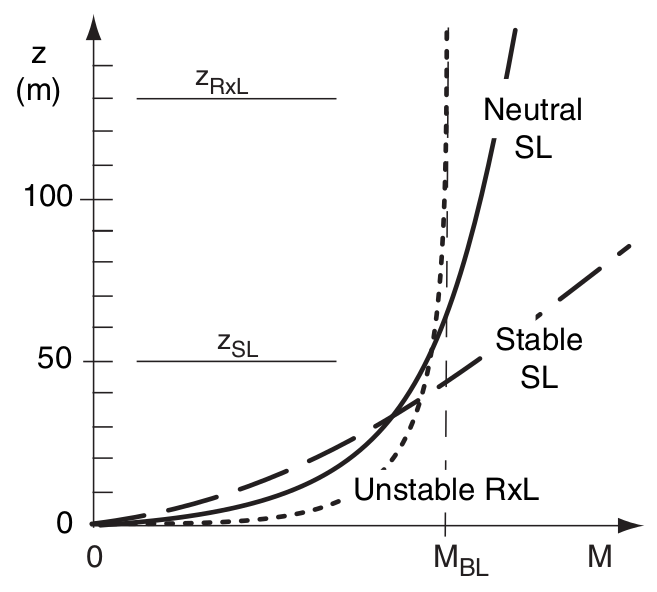
\includegraphics[width=\textwidth]{img/SL_wind.png}  
%@   %Fig 18.20 Stull
%@    %\begin{center}
%@    %\begin{tikzpicture}
%@    %  
%@    %\end{tikzpicture}
%@    %\end{center}
%@\end{columns}
%@ \footnote{donde: $u_*$: velocidad de fricción. $z_0$: coeficiente de rugosidad. $L$: longitud de Monin-Obukhov. $w_*$: Velocidad convectiva.}   
%@\end{frame}
%@
%@
%@
%@
%@\begin{frame}{Longitud de Monin-Obukhov}
%@
%@    Representa la altura (en metros) sobre la cual la producción mecánica de turbulenta es balanceada con la producción de empuje térmico.
%@    $$\boxed{
%@        L=\dfrac{-\rho \,c_p\,T_a\,u_*^3 }{g\,\kappa\,H}
%@        }
%@    $$
%@ 
%@ Está estrechamente vinculado a la estabilidad atmosférica:
%@    \begin{itemize}
%@        \item Estable: $L > 0$ %(since H < 0) very stable: 0 < L < 10
%@        \item Inestable: $L < 0$ %(since H > 0) 
%@        %very unstable: -10 < L < 0
%@        \item Neutra $|L| > 1000$
%@    \end{itemize}
%@    
%@\end{frame}
%@
%@\begin{frame}{Velocidad convectiva}
%@
%@Relacionado a la velocidad vertical de grandes térmicas (remolinos convectivos)
%@
%@Depende de:
%@\begin{itemize}
%@    \item Magnitud de la energia turbulenta convectiva
%@    \item Longitud de escala para los remolinos (i.e. altura de capa de mezcla: $z_i$ )
%@\end{itemize}
%@ 
%@$$\boxed{
%@w_*=\bigg( \dfrac{g\,z_i\,H}{c_p\,\rho\,\theta}\bigg)^{1/3}
%@}
%@$$
%@
%@Valores en el orden de 1-2 m/s
%@
%@\end{frame}
%@
%@
%@
%@\section{Altura de capa de mezcla}
%@
%@\begin{frame}{Altura de capa de mezcla}
%@
%@La altura de capa de mezcla está determinada por dos procesos, los esfuerzos de corte y la convecciòn. Este último solo es importante en atmósferas inestables.
%@    %\begin{figure}
%@    %    \centering
%@    %    \includegraphics[width=0.2\textwidth]{img/scaleHeights.png}
%@    %    \caption{Caption}
%@    %\end{figure}
%@    \begin{center}
%@    \begin{tikzpicture}[scale=0.8, random/.style={decorate,decoration={random steps,amplitude=2pt}}]
%@    \begin{scope}[xshift=-3cm, black!80]
%@       \piso{-2}{2}{0.1}
%@       \draw[random] (-2,2) -- (2,2);
%@       
%@       \draw[latex-latex,xshift=-0.2cm] (-2,0)--(-2,2) node[midway, anchor=east]{$z_{im}$};
%@       
%@       \draw[-latex, very thick] (-0.5,1)--(0.5,1)node[midway,above]{$u_*$};
%@       \node at (0,-0.5) {Estable};
%@    \end{scope} 
%@    
%@    \pause
%@     
%@    \begin{scope}[xshift= 3cm,black!80]
%@      \piso{-2}{2}{0.1}
%@      \draw[random] (-2,2) -- (2,2);
%@      \draw[random] (-2,5) -- (2,5);
%@    
%@      \draw[latex-latex,xshift=0.2cm] ( 2,0)--( 2,5) node[midway, anchor=west]{$z_{ic}$};
%@      
%@      %\node at (0,1){$u_*$};
%@      \draw[-latex, very thick] (-0.5,1)--(0.5,1)node[midway,above]{$u_*$};
%@      \node at (0,3.3){$w_*$};
%@      \node at (0,-0.5) {Inestable};
%@      
%@      \draw[->] (-1.2,2.3) to[out=10,in=-90] (-0.5 ,4.3);
%@      \draw[->] ( 1.2,2.3) to[out=170,in=-90] (0.5 ,4.3);
%@    \end{scope} 
%@    \end{tikzpicture}
%@    \end{center}
%@    
%@Decimos que hay convección \alert{forzada} en el primer caso, y convecciòn \alert{libre} en el segundo.
%@    
%@\end{frame}
%@
%@\begin{frame}{Altura de capa de mezcla}
%@ 
%@Considerando el mezclado \alert{turbulento mecánico}:
%@    $$
%@   \text{En condiciones neutrales:}\qquad  h_{\text{mix}}=\dfrac{0.3 u_*}{|f|}
%@    $$
%@    $$\text{En condiciones estables:}\qquad
%@    h_{\text{mix}}=C\sqrt{\dfrac{ u_* L}{|f|}  }
%@    $$
%@    
%@Bajo condiciones inestables, la $h_{\text{mix}}$ esta principalmente determinada por \alert{mezclado térmico}:
%@    $$\text{En condiciones inestables:}\qquad
%@    h_{\text{mix}}\approx D\sqrt{\dfrac{ u^3_*}{|f|^3L}  }
%@    $$
%@ 
%@\end{frame}
%@

%\section{Turbulencia}
%\begin{frame}{Turbulencia}
%    
%\textit{La turbulencia es parte del flujo no principal que experimenta variaciones abruptas, irregulares, y caóticas.}\\[0.5em]
%
% 
%Es un fenómeno multi-escala, casi exclusivamente tridimensional, de estado transitorio y que  produce \alert{mezcla}.\\[0.5em]
%
%La turbulencia \textbf{no} es una magnitud que se conserva:
%\begin{itemize}
%    \item Es disipada por la \textbf{viscosidad}.
%    \item Es producida y mantenida por: \alert{convección} y \alert{esfuerzos de corte}
%\end{itemize}
%
%
%La turbulencia \textbf{no} se modela, pero sí se estima su contribución a los flujos atmosféricos. 
%Si bien es un fenómeno deterministico, al ser caótico, es común utilizar aproximaciones \alert{estadísticas} para su estudio y modelación.
%
%\end{frame}
%
%\begin{frame}{Turbulencia}{Descomposición de Reynolds}
%
%$$u = \overline{u}+u' $$
%
%\begin{center}
%%\includegraphics[width=0.5\textwidth]{img/reynolds.png}
%\begin{tikzpicture}[scale=0.8]
%\begin{axis}[xshift=-5cm,xlabel=$t$,ylabel=$u$,xmin=0,xmax=8,ymin=-2,ymax=2]
%\addplot[domain=0:8,blue,samples=126,line width=0.7pt] expression{0.01*x+sin(90*x)+0.4*rand};
%\draw[dashed] (0,0)--(3,0)node[above]{$\overline{u}$}--(8,0);
%\draw[<->](5,0)--(5,0.9) node[midway,right]{$u'$};
%\end{axis}
%\end{tikzpicture}
%\end{center}
%
%\end{frame}   
%
%
%\begin{frame}{Turbulencia}{Medidas de turbulencia}
%
%Definición de promedio:
%$$ \overline{u}=\frac{1}{N}\sum_{i=1}^{N} u_i $$
%
%Variancia de velocidad del viento: 
%$$ \sigma_u^2 = \frac{1}{N}\sum_{i=1}^N (\alert{\overline{u} - u_i} )^2$$
%
%Por lo tanto:
%$$ \sigma_u^2= \overline{\alert{u'}^2} $$
%
%Tambien se puede elegir la variancia de otras variables (temperatura, presión, etc.).
%
%
%\end{frame}
%%
%%\setbeamercolor{background canvas}{bg=yellow!10}
%%
%\begin{frame}{Turbulencia}{Turbulent Kinetic Energy (TKE)}
%
%$$
%k = \frac{1}{2} \bigg[ { \sigma_u^2+ \sigma_v^2 + \sigma_w^2} \bigg]
%$$
%
%
%
%$${\displaystyle \underbrace {\frac {\partial k}{\partial t}} _{\begin{smallmatrix}{\text{Local}}\\{\text{derivative}}\end{smallmatrix}}+\underbrace {{\overline {u}}_{j}{\frac {\partial k}{\partial x_{j}}}} _{\begin{smallmatrix}{\text{Advection}}\end{smallmatrix}}=-\underbrace {{\frac {1}{\rho _{o}}}{\frac {\partial {\overline {u'_{i}p'}}}{\partial x_{i}}}} _{\begin{smallmatrix}{\text{Pressure}}\\{\text{diffusion}}\end{smallmatrix}}-\underbrace {{\frac {1}{2}}{\frac {\partial {\overline {u_{j}'u_{j}'u_{i}'}}}{\partial x_{i}}}} _{\begin{smallmatrix}{\text{Turbulent}}\\{\text{transport}}\\{\mathcal {T}}\end{smallmatrix}}+\underbrace {\nu {\frac {\partial ^{2}k}{\partial x_{j}^{2}}}} _{\begin{smallmatrix}{\text{Molecular}}\\{\text{viscous}}\\{\text{transport}}\end{smallmatrix}}\underbrace {-{\overline {u'_{i}u'_{j}}}{\frac {\partial {\overline {u_{i}}}}{\partial x_{j}}}} _{\begin{smallmatrix}{\text{Production}}\\{\mathcal {P}}\end{smallmatrix}}-\underbrace {\nu {\overline {{\frac {\partial u'_{i}}{\partial x_{j}}}{\frac {\partial u'_{i}}{\partial x_{j}}}}}} _{\begin{smallmatrix}{\text{Dissipation}}\\\varepsilon _{k}\end{smallmatrix}}-\underbrace {{\frac {g}{\rho _{o}}}{\overline {\rho 'u'_{i}}}\delta _{i3}} _{\begin{smallmatrix}{\text{Buoyancy flux}}\\b\end{smallmatrix}}}$$
%
%
%%$$
%%\dfrac{\partial k}{\partial t} = \vec{v} \cdot \nabla e + u_*^2 \dfrac{\partial u}{\partial z} + \dfrac{|g|}{T_v}\, H + \varepsilon
%%$$
%
%Convección:
%\begin{itemize}
%    \item Libre: Si $|b| < |\mathcal {P}/3| $
%    \item Forzada Si $|b| > |3\,\mathcal {P}|$
%\end{itemize}
%
%\end{frame}
%
%
%\begin{frame}{Turbulencia}{Número de \alert{Richardson}}
%
%%STULL: The ratio of buoyant energy to shear-kinetic energy is called the bulk Richardson number , Riwhich is dimensionless:
%%JACOBSON: give the ratio of turbulence due to buoyancy relative to that due to shear.
%Es un numero adimensional que mide la relación entre la turbulencia debido a flotación (convectiva) y debido a esfuerzos de corte (mecánica):
%
%$$
%\text{Ri}=\frac{ \text{flotacion}}{\text{esfuerzo cortante}}=\frac{g}{\rho}\frac{\partial \rho /\partial z}{(\partial u/\partial z)^{2}}
%$$
%
%Una versión discretizada muy utilizada es el \alert{Bulk Richardson Number}:
%
%$$
%{\displaystyle R_{B}={\frac {(g/T_{v})\Delta \theta _{v}\Delta z}{(\Delta U)^{2}+(\Delta V)^{2}}}}
%$$
%
%\end{frame}
%
%
%\begin{frame}{Turbulencia}{Covarianza y autocorrelación}
%% Varianza:
%% $$ \mathit{var}(u) = \frac{1}{N} \sum_{i=1}^{N} (u_i -\overline{u})^2$$
% 
% Podemos calcular la covariancia entre dos variables:
%% $$
%\begin{align*}%{ll}
%\mathit{covar}(u,\theta) &= \frac{1}{N} \sum_{i=1}^{N} (u_i -\overline{u})\,(\theta_i -\overline{\theta})\\
%&=\frac{1}{N} \sum_{i=1}^{N} u_i'\,\theta_i' \\
%&= \overline{u'\theta'} 
%\end{align*}
%%$$
%\end{frame}
%
%\begin{frame}{Turbulencia}{Covariancia}
%
%La covarianza mide la cantidad de variación común entre dos variables. 
%
%\begin{tikzpicture}[scale=0.7]
%\begin{axis}[xshift=-5cm,xlabel=$t$,ylabel=$x(t)$,xmin=0,xmax=8,ymin=-2,ymax=2]%Ç,grid=major,grid style={solid}]
%\addplot[domain=0:8,blue,samples=126,line width=0.7pt] expression{-0.4+0.2*x+sin(90*x)+0.4*rand};
%\addplot[domain=0:8,orange!80,samples=126,line width=0.7pt] expression{-0.4+0.2*x+sin(90*x+0.01)+0.4*rand-0.7};
%\end{axis}
%\begin{axis}[xshift=5cm,xlabel=$t$,ylabel=$x(t)$,xmin=0,xmax=8,ymin=-2,ymax=2]%Ç,grid=major,grid style={solid}]
%\addplot[domain=0:8,blue,samples=126,line width=0.7pt] expression{0.2*x+sin(90*x)+0.4*rand};
%\addplot[domain=0:8,orange!80,samples=126,line width=0.7pt] expression{-0.5-(0.2*x+sin(90*x+0.01)+0.4*rand-0.7)};
%\end{axis}
%\end{tikzpicture}
%
%Es positivo si ambas variabeles crecen/decrecen conjuntamente. Es negativa si la variación es opuesta/inversa. Y es cercana a cero si son independientes. 
%
%\end{frame}
%
%%\begin{frame}{Turbulencia}{}
%%
%%Coeficiente de correlación
%%$$ r(u,\theta)= \dfrac{\overline{u'\,\theta'}}{\sigma_u\,\sigma_\theta}$$
%%
%%Es una normalización de la covariación. Vale 1 para variables perfectamente correlacionadas, -1 para variables inversamente-correlacionadas y 0 para variables independientes.
%%
%%\end{frame}
%
%
%\begin{frame}{Turbulencia}{Covarianza y flujos turbulentos}
%    
%    Las covarianzas representan \textbf{ flujos turbulentos}!
%    \begin{center}
%        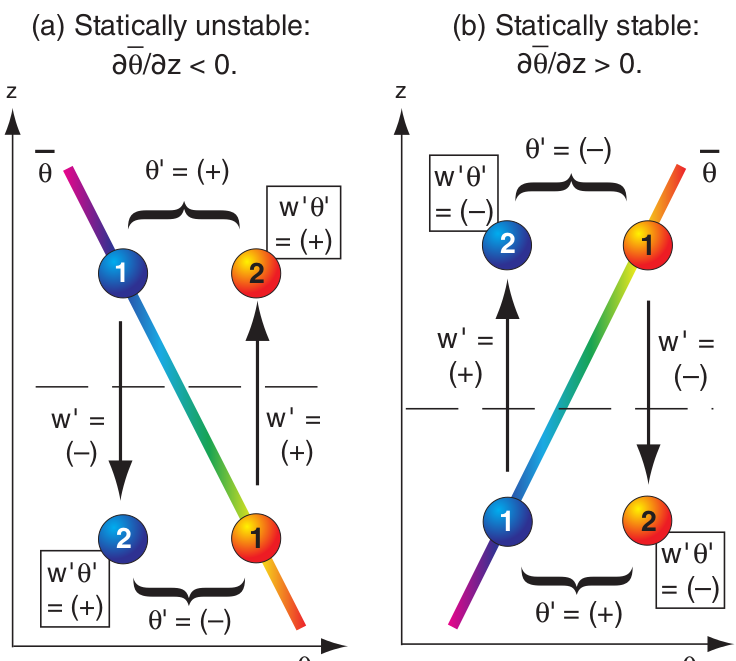
\includegraphics[width=0.4\textwidth]{img/covar_flujo.png}
%    \end{center}
%    
%    $$ \overline{w'\theta'}= F_{H} $$
%    
%\end{frame}
%

%===================================================================================
%SIMILITUD

%\section{Similitud}
%\begin{frame}{Similitud}{}
% 
%Asume que todas las atmósferas se comportan escencialmente de la misma forma pero a distintas escalas.
%Uno de los métodos para construir relaciones entre variables es el \textit{análisis dimensional}. 
% 
%\begin{block}{Teoréma $\pi$ de Buckinham:}
%Dado una problema descrito por un conjunto de ecuaciones de $k$ variables, con $p$ magnitudes fundamentales. Podemos definir $n$ valores adimensionales. Donde:
%$$n= k - p$$
%\end{block}
% 
%\end{frame}
%   
%\begin{frame}{Similitud}
%    Variables que describen el flujo en la capa lìmite: ($u$,$z$,$\rho$,$\nu$,$\tau$)
%    \footnote{ donde        $u$: velocidad del viento,        $z$: altura, $\rho$: densidad del aire, $\nu$: viscosidad (despreciable en régimen turbulento), $\tau$: esfuerzo de corte.}
%    Consideramos $\nu$ despreciable, y definimos la variable \textbf{velocidad de fricción} como:
%    $$ u_* = \sqrt{\frac{|\tau|}{\rho}}$$
%    reduciendo el número de variables a ($u$,$z$,$u_*$), con dos dimensiones, usando el teorema $\pi$-de Buckingham:
%    $$ \pi=\dfrac{z}{u_*}\dfrac{du}{dz}= \text{cte.} = \dfrac{1}{\kappa} \quad\Rightarrow\quad  du = \dfrac{u_*}{\kappa}\dfrac{dz}{z}$$
%    
%    Integrando y despejando $u$ obtenemos:
%    $$ u = \dfrac{u_*}{k} (\ln z + cte.)$$
%    
%\end{frame}
% 
% 
%\begin{frame}{Capa limite}{Perfil de velocidad de viento}
% 
%\begin{itemize}
%    \item Superficie plana, condiciones adiabaticas (neutral):
%    $$ u = \dfrac{u_*}{k} (\ln z + cte.)$$
%    
%    \item Superficie rugosa, condiciones neutral:\footnote{$z_0$: rugosidad de la superficie. Representa la altura extrapolada donde $u=0$}. Asumiendo que $u$ depende de $z/\varepsilon$
%    $$ u = \dfrac{u_*}{k} \bigg[ \ln \dfrac{z}{\varepsilon} - \ln \dfrac{z_0}{\varepsilon} \bigg] \quad\Rightarrow\quad u = \dfrac{u_*}{k} \ln \dfrac{z}{z_0} $$
%    
%%    \item Superficie rugosa, condiciones no neutrales:    
%%    $$ u = \dfrac{u_*}{k} \bigg( \ln \frac{z}{z_0} + 5 \dfrac{z-z_0}{L} \bigg)$$
%\end{itemize}
% 
%\end{frame}
% 
% 
%\begin{frame}{Capa límite}{Perfil de velocidad de viento, Monin-Obukhov}
% 
%Proponen agregar un factor de corrección por calentamiento de la superficie: $\phi(\xi)$ que depende de la estabilidad ($\xi$)
%\begin{columns}
% \column{0.5\textwidth}
% 
%$$
%\dfrac{\kappa z}{u_*}\dfrac{\partial u}{\partial z} = \phi(\xi)
%$$
% 
%Experimentalmente se vio que: 
%$$ \phi(\xi) =\begin{cases}
%    1+4.7 \xi        & \xi > 0  \\
%    1                & \xi = 0  \\
%    (1-15\xi)^{1/4}  & \xi < 0  \\
%\end{cases} 
%$$
% \column{0.5\textwidth}
%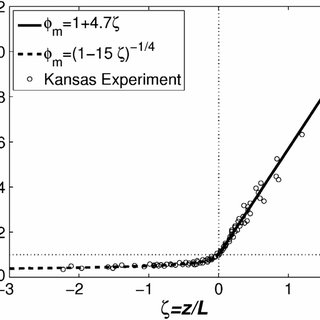
\includegraphics[width=0.7\textwidth]{img/kansas_experiment.jpg}
%\end{columns}
%\end{frame}
% 
% 
%\begin{frame}{Capa límite}{Longitud de Monin-Obukhov}
%El perfil de vientos depende fuertemente de la estabilidad atmosférica. Un indicador de estabilidad propuesto es:
%$$\xi =\dfrac{k\,g\,z \,H}{\rho_0\,c_p\,T_0 \,u_*^3} $$
% 
%depende de $z$, lo que es incombeniente, por eso se definió 
%$$L=z/\xi$$
%por lo tanto:
%$$L =\dfrac{\rho_0\,c_p\,T_0 \,u_*^3}{k\,g\, H} $$
%    
%\end{frame}
% 
% 
% 
% 
%\begin{frame}{Capa límite}{Perfil de velocidad de viento, Monin-Obukhov}
%$$   
%du = \dfrac{u_*}{\kappa} \phi(\xi) \dfrac{dz}{z}
%$$
% 
%Si $\xi > 0$ (estables) hay solución analítica:  
%    $$ u = \dfrac{u_*}{k} \bigg( \ln \frac{z}{z_0} + 5 \dfrac{z-z_0}{L} \bigg)$$
% 
%Para $xi < 0$ (inestable) no hay solución analítica exacta, pero se conoce una aproximación (Benoit, 1977):\footnote{donde $n_0=(1-16z_0/L)^{1/4}$  y $n=(1-16z/L)^{1/4}$}
% 
%$$
%u= \dfrac{u_*}{\kappa} \bigg\{  \ln \frac{z}{z_0} + \ln \bigg[\dfrac{(n_0^2 + 1) \,(n_0 +1)^2}{(n^2 + 1) \,(n +1)^2} \bigg] + 2 [\arctan n - \arctan n_0 ]\bigg\}
%$$
% 
%\end{frame}
% 
% 
% 
% 
% 
% 
% 
% 
% 
% 
% 
% 
% 
% 
% 
%\begin{frame}{Capa límite}{Perfil de temperatura}
% 
%Podemos definir la temperatura potencial de fricción como:
%$$ \theta_* = - \dfrac{H}{\rho c_p u_*}$$
% 
%Escribiendo $L$ en términos de $\theta_*$:
%$$ L = \dfrac{u_*^2\,T_0 }{\kappa \,g\,\theta_*}$$
% 
%De forma análoga a la velocidad se puede calcular los perfiles de temperatura.
% 
%\end{frame}
% 
% 
%\begin{frame}{Balance de calor}{Bajo condiciones estables}
% 
%De la definición de $\theta_*$:
%$$ H = - \rho c_p u_* \theta_* $$
% 
%$$ \theta_* = 0.009(1-0.5n^2)$$
% 
%$$ u = \dfrac{u_*}{k} \bigg( \ln \frac{z}{z_0} + 5 \dfrac{z-z_0}{L} \bigg) = \dfrac{u_*}{k} \bigg( \ln \frac{z}{z_0} + 5 \kappa g \theta_* \dfrac{z-z_0}{T u_*^2} \bigg) $$
% 
%Reordeno, multiplico por $\kappa u_* / \ln(z/z_0)$ y llego a:\footnote{donde $C_D= \kappa / \ln(z/z_0)$}
% 
%$$
%u_*^2 - C_D u \,u_* + C_D u^2 = 0
%$$
%Resuelvo la cuadratica para $u_*$:
% 
%$$
%u_* = \dfrac{C_d u}{2}\bigg[   1 + \sqrt{ \bigg( \dfrac{2\, u}{\sqrt{C_D} u }\bigg)^2 } \bigg]
%$$
% 
%\end{frame}


%\begin{frame}{Turbulencia}{Similitud}
%
%Variables utilziadas en analisis dimensional: ($\sigma_u$,$u_*$,$L$,$h_{\text{mix}}$, $z$). 
%
%En \alert{condiciones neutras ó estables},
%$$\sigma_u = u_* 2.5 \bigg(  1- \dfrac{z}{h_{\text{mix}}}   \bigg)^a
%\qquad
%\sigma_v = u_* 1.9 \bigg(  1- \dfrac{z}{h_{\text{mix}}}   \bigg)^a
%\qquad
%\sigma_w = u_* 1.3 \bigg(  1- \dfrac{z}{h_{\text{mix}}}   \bigg)^a
%$$
%
%En \alert{condiciones inestables}, se define una nueva velocidad de escala convectiva ($w_*$) para contemplar la turbulencia inducida termicamente:
%
%$$ w_* = \bigg( \dfrac{g\,z_i\,H}{c_p\,\rho\,\theta} \bigg) \quad\Rightarrow\quad w_* = \bigg( \dfrac{h_{\text{mix}}}{L\,\kappa}\bigg)^{1/3} $$
%
%Por debajo de la capa de mezcla se obtiene experimentalmente:
%
%$$
%\dfrac{\sigma_u}{w_*}=\dfrac{\sigma_u}{w_*}=\dfrac{\sigma_u}{w_*}=0.6
%$$
% Independientemente de la altura. Por encima de la capa de mezcla la turbulencia decae exponencialmente.
%\end{frame}

%% FIN SIMILITUD
%==============================================================================================
   
   %% Detallado: AERMET y AERMOD, fundamentos.
   %%%=====================================================================================================
%%
%% AERMET:
%%-----------------------------------------------------------------------------------------------------
%\subtitle{AERMET: Fundamentos}
% \begin{frame}{}
%     \maketitle
% \end{frame}
% 
% \begin{frame}{AERMET}{Pre-procesador meteorológico del AERMOD}
%Usa mediciones meteorologicas y computa parámetros de la capa límite que permiten a AERMOD estimar perfiles de vientos, turbulencia y temperatura.
%Los parámetros calculados por AERMET son:
%\begin{itemize}
%\item Flujo de Calor ($H$)
%\item Velocidad de fricción ($ u* $)
%\item Longitud de Monin-Obukhov ($L$)
%\item Escala de velocidad convectiva ($ w* $)
%\end{itemize}
%
%%El crecimiento y estructura de la CLP está regulada por los flujos de calor y momentum que a su vez dependen de efectos de la superficie. El espesor de esta capa está incluenciada a escala local por características de la superficie: rugosidad ($z0$), albedo ($a0$), y disponibilidad de humedad ($b0$).
%
%Además estima alturas de mezcla mecánica ($z_{im}$) y convectiva ($z_{ic}>$). Y define la estabilidad de la CLP por el signo de $H$ (convectiva si H>0 y estable si H<0).
%%
%\end{frame}
%
%\begin{frame}{AERMET}{Archivos de salida}
%
%El AERMET genera dos archivos de salida:
%
%
%\begin{columns}[t]
%\column{0.5\textwidth}
%\texttt{*.SFC}
%\begin{table}
%\small
%\centering
%\begin{tabular}{c| l}
%1-5             & fecha y hora \\
%6               & H (W/m 2) \\
%7               & $u_*$ (m/s) \\
%8               & $w_*$ (m/s) \\
%9               & $d\theta/dz$ (K/m) \\
%10              & $z_{ic}$ (m) \\
%11              & $z_{im}$ (m) \\
%12              & $L$ Monin-Obukhov (m)\\
%13-15           & $z_0$, $b_0$, $a_0$\\
%    16-27           & datos usados (u,T,ppt,p,etc.)\\
%%16-18           & $u$ \\
%%19-20           & $T$ \\
%%21-22           & precipitación \\
%%23              & humedad relativa \\
%%24              & presión \\
%%25              & cobertura de nubes \\
%%26              & $u$ ajustado \\
%%27              & flag interpolacion \\
%\end{tabular}
%\end{table}
%
%\column{0.5\textwidth}
%    
%\texttt{*.PFL}
%\begin{table}
%\small
%\centering
%\begin{tabular}{c| l}
%1-4         &  fecha y hora  \\
%5           &  altura de medicion (m)  \\
%6           &  indicador: 1/0 (ultimo nivel)\\
%7-8         &  direccion y velocidad de viento \\
%9           &  temperatura \\
%10          &  $\sigma_\theta$ - desvio de dirección del viento\\
%11          &  $\sigma_w$ desvio de velocidad del viento
%    \end{tabular}
%\end{table}
%\end{columns}
%    
%\end{frame}
%
%
%
% 
%\begin{frame}{Balance de energía}{Cálculo de calor sensible \footnote{$R_n$: radiación neta. $H$: calor sensible. $\lambda E$: calor latente. $G$: flujo de calor al suelo.}}
% 
%\begin{center}
%\begin{tikzpicture}[scale=0.5]
%    \begin{scope}
%    \piso{-3}{3}{0}
%    \draw[-latex,very thick] (-2.5, 2.0) -- (-2.0, 0.0) node[midway,anchor=east]{$\mathrm{R_n}$} ;
%    \draw[-latex,very thick] (-1.0, 0.0) -- (-0.5, 2.0) node[midway,anchor=west]{$\lambda \mathrm{E}$  };
%    \draw[-latex,very thick] ( 0.0, 0.0) -- ( 0.0,-1.0) node[midway,anchor=west]{$\mathrm{G}$  };
%    \draw[-latex,very thick] ( 1.0, 0.0) -- ( 1.5, 2.0) node[midway,anchor=west]{$\mathrm{H}$  };
%    \end{scope}
%\end{tikzpicture}
%\end{center}
%\vspace{-0.5em}
%$$ R_n = H + \lambda E + G$$
% 
%Considerando:\footnote{$B_0$: Relación de Bowen, depende del tipo de cobertura.}
%$$ G \approx 0.1 R_n \qquad B_0 =\dfrac{\lambda E}{H}  $$
% 
%El calor sensible (H) se puede calcular como:
%$$ 
%H = \dfrac{0.9\,R_n}{ 1 + 1/B_0}
%\qquad
%\begin{cases}
%    H<0  & \text{Flujo atmosfera a superifice (ESTABLE)}  \\
%    H=0  & \text{No hay flujo neto (NEUTRO)}  \\
%    H>0  & \text{Flujo superficie a atmosfera (INESTABLE)}
%\end{cases}
%$$
%\end{frame}
% 
%\begin{frame}{Balance Radiativo}{Radiación Neta}
% 
%\begin{center}
%\begin{tikzpicture}[scale=0.9]
%    \begin{scope}
%    \piso{-3}{3}{0}
%    \draw[-latex,very thick] (-2.5, 2.0) -- (-2.0, 0.1) node[midway,anchor=east]{\small$\mathrm{R}$} ;
%    \draw[-latex,very thick] (-1.8, 0.1) -- (-1.3, 2.0) node[midway,anchor=west]{\small$rR$};
%    \draw[-latex,very thick] (-0.5, 2.0) -- (-0.5, 0.1) node[midway,anchor=west]{\small$c_1T^6$};
%    \draw[-latex,very thick] ( 1.0, 0.1) -- ( 1.0, 2.0) node[midway,anchor=west]{\small$\sigma T^4$};
%    \draw[-latex,very thick] ( 2.5, 1.5) -- ( 2.5, 0.2) node[midway,anchor=west]{\small$c_2\,n$};
%    
%    \draw[scale=0.4,xshift=7cm, yshift=4cm] (-1.6,-0.7) .. controls (-2.3,-1.1) and (-2.7,0.3) .. (-1.7,0.3) .. controls (-1.6,0.7)and (-1.2,0.9) .. (-0.8,0.7) .. controls (-0.5,1.5) and (0.6,1.3) .. (0.7,0.5) .. controls (1.5,0.4) and (1.2,-1) .. (0.4,-0.6) .. controls (0.2,-1) and (-0.2,-1) .. (-0.5,-0.7) .. controls (-0.9,-1) and (-1.3,-1) .. cycle;
% 
%    \end{scope}
%\end{tikzpicture}
%\end{center}
% 
%$$ R_n = \dfrac{R - r\,R + c_1 T^6 + c_2 \,n - \sigma T^4}{1 + c_3} $$
% 
% 
% 
%donde:
%\begin{itemize}
%    \item $R - rR    $ : Radiación incidente menos albedo.
%    \item $c_1 T^6   $ : Absorción de GEIs.
%    \item $\sigma T^4$ : Emisión de superficie (Stephan-Boltzman).
%    \item $c_2 \, n  $ : Emisión de las nubes.
%\end{itemize}
% 
%\end{frame}
% 
% 
%\begin{frame}{Balance Radiativo}{Radiación incidente}
%  
%\begin{center}
%\begin{tikzpicture}[scale=0.9]
%    
%    \draw[fill=black!10,scale=0.4,xshift=0cm, yshift=3cm] (-1.6,-0.7) .. controls (-2.3,-1.1) and (-2.7,0.3) .. (-1.7,0.3) .. controls (-1.6,0.7)and (-1.2,0.9) .. (-0.8,0.7) .. controls (-0.5,1.5) and (0.6,1.3) .. (0.7,0.5) .. controls (1.5,0.4) and (1.2,-1) .. (0.4,-0.6) .. controls (0.2,-1) and (-0.2,-1) .. (-0.5,-0.7) .. controls (-0.9,-1) and (-1.3,-1) .. cycle;
%    \piso{-2}{1}{0}
%    \draw[-latex,very thick] (-1.5, 2.0)--(0.0, 0.0) node[midway,anchor=east]{$\mathrm{R}$} ;
%    
%    \coordinate (O) at (0,0);
%    \coordinate (A) at (-1,0) ;
%    \coordinate (B) at (-1.5,2);
%    \pic[draw,black,  angle eccentricity=1.5]{angle=B--O--A} node[anchor=south east,xshift=-10pt] {$\phi$};
%    
%    %sol:
%   \fill[yellow!30](-1.7,2.2) circle[radius=.25cm];
%   \fill[orange!60](-1.7,2.2) circle[radius=.2cm];
% 
%\end{tikzpicture}
%\end{center}
% 
%Holtslag y Ulden (1983):\footnote{donde Ángulo de Elevación Solar: $\phi=\arcsin (sin\lambda \sin\delta + \cos\lambda\cos\delta\cosh)$, con $\lambda$:latitud, $\delta$: declinación, y h el ángulo horario. Fracción nubosa: $n$.}
%$$  R = (990 \sin(\phi) - 30 ) \, (1-0.75 n^{3.4}) $$
% 
%\end{frame}
% 
% 
%
%\begin{frame}{Caracterización de CLP}{Similitud}
%    
%\end{frame}
%
%
%\begin{frame}{Caracterización de CLP}{Velocidad de fricción}
%    
%    
%    $$
%    u_*=\sqrt{\dfrac{\tau}{\rho}}
%    $$
%    
%
%\end{frame}
%
%\begin{frame}{Caracterización de CLP}{Longitud de Monin-Obukhov}
%
%    Representa la altura (en metros) sobre la cual la produccion mecánica de turbulenta es alanceada con la producción de empuje térmico.
%    $$
%        L=\dfrac{-\rho \,c_p\,T_a\,u_*^3 }{g\,\kappa\,H}
%    $$
% 
%    \begin{itemize}
%        \item Estable: $L > 0$ %(since H < 0) very stable: 0 < L < 10
%        \item Inestable: $L < 0$ %(since H > 0) 
%        %very unstable: -10 < L < 0
%        \item Neutra $|L| > 1000$
%    \end{itemize}
%    
%\end{frame}
%
%\begin{frame}{Caracterización de CLP}{Velocidad convectiva}
%    Related to the vertical velocities in the large
%thermals (i.e., convective eddies)
%Depende de:
%\begin{itemize}
%    \item Magnitude of buoyant turbulent energy
%    \item Scaling height for the eddies (i.e., z i )
%\end{itemize}
% 
% 
%$$
%w_*=\bigg( \dfrac{g\,z_i\,H}{c_p\,\rho\,\theta}\bigg)^{1/3}
%$$
%Valores en el orden de 1-2 metros/segundo
%
%\end{frame}
%
%
%\begin{frame}{Caracterización de CLP}{Perfiles}
%    AERMOD usa relaciones de similitud y observaciones meteorológicas para construir perfiles de viento, temperatura y turbulencia, hasta los 4000 metros en cada hora modelada.
%    
%    
%\end{frame}
%
%\begin{frame}{Caracterización de CLP}{Variables effectivas}
%    
%\end{frame}
%
%%$$
%%
%%Nos queda como incognita la radiación neta R<sub>n</sub> que puede ser observada o estimada.
%%
%%La radiación incidente para cielos claros (R0) está dado por:
%%
%%$$ R_0 = a_1 \sin \phi + a_2 $$
%%
%%Podemos llegar a:
%%
%%$$ R_n = \dfrac{(1- r_{(\phi)}) R + c_1 T^6_{\text{ref}} - \sigma_{SB}T^4_{\text{ref}} - c^2\,n }{1 + c_3} $$
%%
%%
%%
%%\begin{frame}{Estimaciones para atmósfera convectiva}{Balance radiativo}
%%    
%%\end{frame}
%%#### Velocidad de fricción y Longitud de Monin-Obukhov
%%
%%Una vez que se estima el flujo de calor (H), AERMET estima la $u^*$, $L$ mediante un método iterativo, usando las siguentes expresiones:
%%
%%
%%$$
%%u_* = \dfrac{\kappa \,u}{  \ln(z_{\text{ref}}/z0) - \Psi_m(z_{\text{ref}}/L) + \Psi_m(z_{\text{0}}/L)  }
%%$$
%%
%%y 
%%
%%$$ L =-\dfrac{\rho c_p T u_*^3}{\kappa g H} $$
%%
%%
%%
%%$$ \Psi_m (z_0/L) = 2\ln(\dfrac{1+\mu_0}{2})+\ln(\dfrac{1+\mu_0^2}{2}) - 2\tan^{-1}(\mu_0) + 0.5\,\phi $$
%%
%%
%%$$ \Psi_m (z_0/L) = 2\ln(\dfrac{1+\mu_0}{2})+\ln(\dfrac{1+\mu_0^2}{2}) - 2\tan^{-1}(\mu_0) + 0.5\,\phi $$
%%
%%
%%donde 
%%<center>
%%&mu;<sub></sub> = (1 -16 z<sub>ref</sub> / L )<sup>1/4</sup>
%%
%%&mu;<sub>0</sub> = (1 -16 z<sub>0</sub> / L )<sup>1/4</sup>
%%</center>
%%
%%El proceso requere un $u_*$ inicial, que se calcula contemplando los $\Psi$ igual a cero, y luego la iteración continua hasta que los valores de L difieren en menos del 1%.
%%
%%
%%
%%\begin{frame}{Estimaciones para atmósfera convectiva}{Altura de mezcla}
%%    
%%\end{frame}
%%#### Alturas de mezcla:
%%
%%
%%$$
%%z_{ic} \theta(z_{ic}) - \int_0^{z_{ic}} \theta(z) \,dz = (1 + 2A) \int_0^t \dfrac{H(t')}{\rho c_p} dt
%%$$
%%
%%donde &theta;<sub>0</sub>(z) es la distribución vertical de la temperatura potencial dado por el sondeo de la mañana y el término derecho representa el flujo de calor acumulado en z=0. A=0.2
%%
%%Una vez que conocemos z<sub>ic</sub> podemos obtener $w_*$ como:
%%
%%$$
%%w_* = (\dfrac{gHz_{ic}}{\rho c_p T})^{1/3}
%%$$
%%
%%
%
%
%%### Estimación para atmosfera estable
%%\begin{frame}{Estimaciones para atmósfera estable}{Balance radiativo}
%%    
%%\end{frame}
%%Para el caso de atmosferas estables los calculos son más simples y no requieren procesos iterativos
%%
%%
%%
%%Usando
%%<center>
%%H=-D c<sub>p</sub> u<sub>*</sub> &theta;<sub>*</sub>
%%</center>
%%
%%Luego:
%%
%%$$ \kappa \dfrac{u}{u_*} = \ln( \dfrac{z_{\text{ref}}}{z0} ) + \beta_m \dfrac{z_{\text{ref}}}{L}  $$
%%
%%
%%\begin{frame}{Estimaciones para atmósfera estable}{Velocidad de fricción}
%%    
%%\end{frame}
%
%
%%La velocidad de fricción se calcula como:
%%
%%$$ u_* = C_D u/2 (1 + \sqrt{1- (2u_0/\sqrt{C_D} u)^2} ) $$
%%
%%donde 
%%
%%$$ C_D \dfrac{\kappa}{\ln{z_{\text{ref}}/z_0}} $$
%%
%%y 
%%
%%$$ u_0 = \sqrt{\beta_m z_{\text{ref}} g \theta_* / T} $$
%%
%%
%%$$ \theta_* = 0.09 (1-0.5n^2) $$
%%
%%donde $n$ es la fracción opaca por cobertura nubosa.
%%
%%El flujo de calor se computa como :
%%
%%$$H=-\rho c_p u_* \theta_* $$
%%
%%con $ u_* = \hat{u}_* u / \hat{u}_* $ y $ \theta_* =\hat{theta}_* u / \hat{theta}_*$
%%
%%y 
%%
%%$$ z_{im} = 2300 u_*^{3/2} $$
%%
%
%
%
%
%
%
%
%
%\begin{frame}{Turbulencia}{Similitud}
%Variables utilziadas en analisis dimensional: ($\sigma_u$,$u_*$,$L$,$h_{\text{mix}}$, $z$). 
%
%En \alert{condiciones neutras}
%$$
%\sigma_u = u_* 2.5 \,e^{-1.5 \frac{z}{h_{\text{mix}}}}   \bigg)^a
%\qquad
%\sigma_v = u_* 1.6 \bigg(  1- \dfrac{z}{h_{\text{mix}}}  \bigg)^a
%\qquad
%\sigma_w = u_* 1.25 \bigg(  1- \dfrac{z}{h_{\text{mix}}} \bigg)^a
%$$
%
%En condiciones \alert{estables},
%$$
%\sigma_u = u_* 2.2   \bigg(  1- \dfrac{z}{h_{\text{mix}}}   \bigg)^a
%\qquad
%\sigma_v = u_* 2.2 \bigg(  1- \dfrac{z}{h_{\text{mix}}}   \bigg)^a
%\qquad
%\sigma_w = u_* 1.73 \bigg(  1- \dfrac{z}{h_{\text{mix}}}   \bigg)^a
%$$
%\end{frame}
%
%\begin{frame}{Turbulencia}{Similitud}
%En \alert{condiciones inestables}, se define una nueva velocidad de escala convectiva ($w_*$) para contemplar la turbulencia inducida termicamente:
%
%$$ w_* = \bigg( \dfrac{g\,z_i\,H}{c_p\,\rho\,\theta} \bigg) \quad\Rightarrow\quad w_* = \bigg( \dfrac{h_{\text{mix}}}{L\,\kappa}\bigg)^{1/3} $$
%
%Por debajo de la capa de mezcla se obtiene experimentalmente:
%
%$$
%\dfrac{\sigma_u}{w_*}=\dfrac{\sigma_u}{w_*}=\dfrac{\sigma_u}{w_*}=0.6
%$$
% Independientemente de la altura. Por encima de la capa de mezcla la turbulencia decae exponencialmente.
%\end{frame}
%
%
%
%
%\begin{frame}{Altura de capa de mezcla}
% 
%Considerando el mezclado \alert{turbulento mecánico}:
%    $$
%   \text{En condiciones neutrales:}\qquad  h_{\text{mix}}=\dfrac{0.3 u_*}{|f|}
%    $$
%    $$\text{En condiciones estables:}\qquad
%    h_{\text{mix}}=C\sqrt{\dfrac{ u_* L}{|f|}  }
%    $$
%    
%Bajo condiciones inestables, la $h_{\text{mix}}$ esta principalmente determinada por \alert{mezclado térmico}:
%    $$\text{En condiciones inestables:}\qquad
%    h_{\text{mix}}\approx D\sqrt{\dfrac{ u^3_*}{|f|^3L}  }
%    $$
% 
%\end{frame}
%
%
%
%
%=====================================================================================================
%
% AERMOD:
%-----------------------------------------------------------------------------------------------------
\subtitle{AERMOD: Fundamentos}
 \begin{frame}{}
     \maketitle
 \end{frame}
 
\begin{frame}{AERMOD}{Sistema de modelado}
 
 \begin{center}
 \begin{tikzpicture}[
    programa/.style={draw, minimum width=2cm, minimum height=1.2cm },
    archivo/.style={draw, minimum height=3.7em, minimum width=3em, fill=white, copy shadow={shadow xshift=2pt, shadow yshift=2pt, black!30, draw}},]

\begin{scope}[scale=0.3]
       
    %ARCHIVOS:
   \node[archivo,              , align=center] (dem) {MDE\\\texttt{.tiff}};
   \node[archivo, below= 0.2cm of dem, align=center ] (ish) {\texttt{.sam}\\\texttt{.ish}};
   \node[archivo, below= 0.2cm of ish, align=center ] (fsl) {\texttt{.fsl}};
   \node[archivo, below= 0.2cm of fsl, align=center] (lu)  {LU\\\texttt{.tiff}};
   
    %PROGRAMAS:
   \node[programa, right = 3cm of ish          ] (aermet) {AERMET};
   \node[programa, right = 2cm of aermet, fill=blue!10] (aermod) {\textbf{AERMOD}};
   \node[programa, above = 0.5cm of aermet,fill=yellow!20] (aermap) {AERMAP};
   \node[programa, right = 2.65cm of lu        ](aersurface) {AERSURFACE};
   \node[programa, below = 2.3 cm of aermod,fill=yellow!20](bpip) {BPIPPRM};
   
   %variables:
   \node[red!80, below = -0.5cm of aermet, align=center] {\small $u_*$,$w_*$,$H$,$L$\\\small$d\theta/dz$,$z_{ic}$,$z_{im}$\\\small $\sigma_w$, $\sigma_\theta$};
   \node[red!80, below = -0.5cm of aersurface] {\small $a_0$,$b_0$,$z_0$};
   \node[red!80, below = -0.5cm of aermap] {\small $z_r$,$z_h$,$z_p$};
   \node[red!80, below = -0.5cm of bpip, align=center] {\small $b_{len}$,$b_{hgt}$,$b_{wid}$\\,$x_{badj}$,$y_{badj}$};
   
   %Flechitas
   \draw[-latex,thick,black!60] (aersurface.north) -- (aermet.south) node[midway,left]{\small\texttt{.out}};
   \draw[-latex,thick,black!60] (ish.east) edge (aermet.west);
   \draw[-latex,thick,black!60] (fsl.east) edge ([yshift=-0.3cm] aermet.west);
   \draw[-latex,thick,black!60] (lu.east) edge (aersurface.west);
   \draw[-latex,thick,black!60] (dem.east) edge (aermap.west);
   \draw[-latex,thick,black!60] (aermap.east) -- ([yshift=3cm] aermod.north)--(aermod.north) node[midway,right]{\small\texttt{.rou}};
   \draw[-latex,thick,black!60] (aermet.east) -- (aermod.west) node[midway,below]{\texttt{.pfl}} node[midway,above]{\texttt{.sfc}};
   \draw[-latex,thick,black!60] (bpip.north) -- (aermod.south) node[midway,right]{\small\texttt{.out}};
\end{scope}
\end{tikzpicture}
\end{center}

\end{frame}


\begin{frame}{AERMOD}{Características generales}
    
    \begin{itemize}
        \item Modelo de pluma gaussiano de estado estacionario.
        \item Usa parametrización continua para los coeficientes de dispersión ($\sigma_{y,\,z}$).
        \item Caracteriza la capa límite, usando la teoria de similitud para representar las variables en el perfil de esta.
        \item Contempla inhomogeneidades de la PBL mediante el uso de \textit{variables efectivas}.
        \item Representa la dispersión en terrenos complejos.
        \item Contempla corrientes ascendentes y descendentes mediante una distribución vertical bi-gaussiana.
        \item Representa \textit{plume lofting} y la inyección de plumas flotantes a capas estables.
    \end{itemize}
\end{frame} 

\section{Interfaz meteorológica}
\begin{frame}{Cálculo de perfiles}{Perfil de viento}

Sigue el típico patron logarítmico:
$$
u(z) = \begin{cases}
    u_(z_i) & z > z_i  \\
     \dfrac{u_*}{\kappa} \bigg[ \ln{\dfrac{z}{z_0}} - \Psi(z/L) + \Psi(z_0/L )\bigg]&  7z_0 < z < z_i\\[0.8em]
    \dfrac{z}{7\,z_0}u_{(7z_0)} & z < 7z0  \\[0.8em]
\end{cases}
$$
Para condiciones \alert{estables}:
$$ 
\Psi(\frac{z}{L}) = 17 \exp\bigg(-0.29\dfrac{z}{L}\bigg)
$$
 
 En condiciones \alert{inestables}:
 $$
 \Psi( \frac{z}{L}) =  2\,\ln \frac{2 - 16\,z/ L}{2} + \ln \frac{1+(1 - 16\,z/L)^2}{2} - 2 \arctan( (1 - 16\,z / L) + \pi/2 )
 $$
   
\end{frame}

%\begin{frame}{Cálculo de perfiles}{Gradiente de temperatura potencial}
%
%Para condiciones \alert{estables} se calcula:
%    $$
%     \dfrac{\partial \theta}{\partial z} (z)=
%     \begin{cases}
%       % \dfrac{\theta_*}{k(2)}\bigg( 1+ 5 \dfrac{2}{L}\bigg) &  z < 2m\\[0.8em]
%        \dfrac{\partial \theta}{\partial z}\bigg\rvert_{100} \exp{ \bigg[ - \dfrac{z-100}{0.44\,z_{i\,\theta}} \bigg] } & z >100m \\[1em]
%        \dfrac{\theta_*}{k\,z}\bigg( 1+ 5 \dfrac{z}{L}\bigg) & 2m < z < 100m  \\[0.8em]
%        \dfrac{\partial \theta}{\partial z} \bigg\rvert_{2}  &  z < 2m\\[0.8em]
%    \end{cases}
%    $$
% Bajo condiciones \alert{inestables} se asume que el gradiente es constante:
% $$\dfrac{\partial \theta}{\partial z} = 0 $$
% \end{frame}
% 
%\begin{frame}{Cálculo de perfiles}{Temperatura potencial}
% 
% Una vez conocido el perfil del gradiente de la temperatura potencial, se puede calcular la temperatura potencial como:
% 
% $$
% \theta(z+\Delta z) = \theta(z) + \dfrac{\partial \theta}{\partial z}\bigg\rvert_{z} \Delta z
% $$
% 
% Para esto es necesario conocer $\theta$ en algun punto de referencia:
% 
% $$
% \theta_{ref} =T_{ref}+\dfrac{g}{c_p}\,z_{mls}
% $$
% 
% donde: 
% $$z_{mls}=z_{ref}+z_{base}$$
%\end{frame}
%
%\begin{frame}{Cálculo de perfiles}{Coeficiente turbulento vertical}
%    
%Se puede separar en una componente convectiva y otra mecánica:
%    $$ 
%    \sigma_w^2 = \sigma_{wc}^2 + \sigma_{wm}^2
%    $$
%    
%    
%    $$
%    \sigma_{w\,c}^2 = 1.6\, w_*^2\, \bigg(\dfrac{z}{z_i}\bigg)^{2/3} \qquad \sigma_{w\,m}^2 =1.3u_*\sqrt{1-\dfrac{z}{z_i}}
%    $$
%    
%\end{frame}

%\begin{frame}{Cálculo de perfiles}{Coeficiente turbulento vertical}
%    También se puede separar en una componente convectiva y otra mecánica:
% 
%     $$ 
%     \sigma_{v\,c}^2 = \sigma_{vc}^2 + \sigma_{vm}^2
%     $$
%     
%     $$
%     \sigma_{v\,m}^2 = 0.35\,w_*^2 \qquad \sigma_v^2 = 3.6 \, u_*^2
%     $$
%     
%    
%\end{frame}


\begin{frame}{Cálculo de variables efectivas}
 
% Las plumas se extienden en todo el espacio, pero los parámetros de la pluma solo pueden tomar un valor para representar la atmósfera, aunque estas cambien en el espacio. Esto es una fuente de error pero puede reducirse usando valores adecuados promedios para asegurar la representatividad.
 
El proceso de calcular variables efectivas puede resumirse en:
\begin{itemize}
 \item Cálculo de altura del centroide de la pluma ($h_c$) 
 \item Cálculo de $\sigma_z$ en base a los valores de $\sigma_w$ y $h_c$
 \item Se considera el menor de los intervalo entre $h_c$ y el receptor ($z_r$) ó entre $h_c$ y $2.15\sigma_z$ en la dirección del receptor.
 \item La variable de interés es integrada entre el intervalo vertical definido en el paso previo y dividido por el dicho intervalo para obtener la variable efectiva.
\end{itemize}

Por ejemplo, la velocidad efectiva: \footnote{No confundir con la velocidad promedio $\overline{u}=1/z_i \, \int_0^{z_i} u(z) dz$}
    $$\tilde{u} = \dfrac{1}{h_c - z_r} \int_{z_r}^{h_c} u(z) dz $$
    
\end{frame}

    


\section{Cálculo de concentraciones}
 
\begin{frame}[t]{Terreno complejo}{}
 
 AERMOD calcula dos plumas: una ignorando el terreno y otra siguiendo el terreno.
  
\begin{center}
\begin{tikzpicture}[scale=1]
\ejesXZ{-5}{0}{0.45}
\piso{-4}{4.5}{0}
\chimenea{-3.1}{0}{0.2}{1}
%pluma real
\fill[red!20,opacity=0.5] (-3,1) -- (4,2) -- (4,0.4) -- (-3,1);
%mountain
\draw[ latex-latex] (-3.2, 1)--(-3.2,0) node[midway, anchor=east]{$h_s$};
 
     \node[brown] at (0.5,0.8) {\textbullet};
     \fill[fill=blue] (0.5,1.1) circle[radius=2pt] node[left]{$r_1$};
     \fill[fill=red ] (0.5,0.3) circle[radius=2pt] node[left]{$r_2$};
     
     \draw[latex-latex] (0.5,0.8)--(0.5,1.1)node[midway,anchor=west]{$z_{p}$}; 
     \draw[latex-latex] (0.5,0.0)--(0.5,0.3)node[midway,anchor=west]{$z_{p}$}; 
    % \draw[latex-latex] (1.5,0.0)--(1.5,1.1)node[midway,anchor=west]{$z_{r}$};
    % \draw[latex-latex] (1.0,0.0)--(1.0,0.8)node[midway,anchor=west]{$z_{t}$}; 
     
   \draw[orange!70, dashed] (-3,0.85)--(5,0.85) node[anchor=west]{$H_c$};
   \draw[|-|, green] (4.0,0.85)--(4.0,2.0) node[midway, anchor=west]{$M_a$};
   \draw[|-|, green] (4.0,0.85)--(4.0,0.5) node[midway, anchor=west]{$M_b$};
   \draw[clip]
    decorate [decoration={random steps,segment length=3pt,amplitude=1pt}]%
    {(-1,0) --(0,0.3)-- (0.5,0.8) -- (1,1.5)--(2,2) --(3.0,2.5)-- (3.5,2.3) -- (4,0)}-- (0,0) -- (-1,0);
    \fill[rock](-1,0) rectangle (4,4);
        
\end{tikzpicture}
\end{center}
 
 la concentración final es la suma ponderada de estas dos: \footnote{donde $f=0.5 + 0.5 \varphi_p $ y $\varphi_p= M_b / M_a\,M_b$. $M_a$ Masa sobre $H_c$ y $M_b$ masa por debajo de $H_c$. $H_c$: critical dividing streamline, depende de $h_c$: hill slope scale (calculado en AERMAP).}

  $$ C_{tot} = f {\color{blue} C_{ref} } + (1-f) {\color{red}C_{terr.} } $$



\end{frame}
 
 
\begin{frame}{Cálculo de dispersión}{Fórmula general}

    $$
        \overline{c} = \dfrac{Q}{\tilde{u}}\,\varphi_y\,\varphi_z
    $$
    
$\varphi_y$ es la dispersión horizontal:
$$
\varphi_y =\dfrac{1}{\sqrt{2\pi}\sigma_y}\exp{\bigg(-\dfrac{1}{2}\dfrac{y^2}{\sigma_y^2}\bigg)}
$$

la dispersión vertical $\varphi_z$ tambien tiene forma \textit{gaussiana} en \alert{atmósferas estables}:
$$
\varphi_z =\dfrac{1}{\sqrt{2\pi}\sigma_z} \bigg\{ \exp{\bigg[-\dfrac{1}{2}\dfrac{(z+h_c)^2}{\sigma_z^2}\bigg]} + \exp{\bigg[-\dfrac{1}{2}\dfrac{(z-h_c)^2}{\sigma_z^2}\bigg]} \bigg\}
$$

%\footnote{
donde $h_c$ es la altura del centro de la pluma. 
$$h_c=h_s + \Delta z$$
%}
\end{frame}
 
 
 
\begin{frame}{Cálculo de dispersión}{Elevación de la pluma (\textit{plumerise})}
    
    La elevación se calcula usando los flujos de momentum ($F_m$) y empuje ($F_b$)\footnote{ donde $F_m=w_s^2\,r_s^2 T/T_s$ y $F_b=g\,w_s\,r_s^2 \Delta T/T_s$ }
  
  $$ \Delta z = \bigg( \dfrac{3\,F_m\,x}{0.36\,u_{(h_s)}^2} + \dfrac{3\,F_b\,x}{0.72\,u_{(h_s)}^3} \bigg)^{1/3}$$
 \begin{center}
  \begin{tikzpicture}
      \ejesXZ{-5}{0}{0.45}
      \piso{-4}{4.5}{0}
      \chimenea{-3.1}{0}{0.2}{1}
       \fill[red!20,opacity=0.5] plot[domain=-3:4,samples=40]({\x},{1+(\x+3)^(1/3)+(\x+3)*0.1})--++(0,-2)--plot[domain=4:-3,samples=40]({\x},{1+(\x+3)^(1/3)-(\x+3)*0.1});
       \draw[thick, black!60,dashed] plot[domain=-3:4.1,samples=60]({\x},{(\x+3)^(1/3)+1}) node[right]{$h_s + \Delta z$};
      \draw[| latex-latex] (-3.2, 1)--(-3.2,0) node[midway, anchor=east]{$h_s$}; 
 \end{tikzpicture}
 \end{center}
    
\end{frame}
 



\begin{frame}{Cálculo de dispersión}{Updrafts y Downdrafts}
 
 Bajo condiciones \alert{inestables} hay corrientes verticales ascendentes y descendentes:
 
 \begin{center}
 \begin{tikzpicture}[scale=1.0]
 \ejesXZ{-5}{0}{0.45}
 \piso{-4}{4.5}{0}
 \chimenea{-3}{0}{0.2}{1.2}
 %pluma real
 \fill[red!20,opacity=0.5] (-2.8,1.2) to[out=40 ,in=180] 
                           (-2. ,1.7) to[out=-10,in=180]
                           (0.2 ,0.8) to[out=10 ,in=180]
                           (1.2 ,1.7) to[out=  0,in=180]
                           (3.2 ,1.0) to[out=10 ,in=200]
                           (4.5 ,1.5) -- 
                           (4.5 ,3.7) to[out=220 ,in= 10]
                           (3.0 ,2.2) to[out=180 ,in=  0]
                           (1.0 ,2.8) to[out=200 ,in= 10]
                           (0.0 ,1.3) to[out=160 ,in=  0]
                           (-2. ,2.0) to[out=180 ,in= 40] (-3.0,1.2);
 %\draw[ latex-latex] (-3.2, 1.2)--(-3.2,0) node[midway, anchor=east]{$h_s$};
         
 \draw[dashed,black!50] (-3.0, 0.0)--++(0,3.5);
 \draw[dashed,black!50] (-2.0, 0.0)--++(0,3.5);
 \draw[dashed,black!50] ( 0.0, 0.0)--++(0,3.5);
 \draw[dashed,black!50] ( 1.0, 0.0)--++(0,3.5);
 \draw[dashed,black!50] ( 3.0, 0.0)--++(0,3.5);
 \draw[dashed,black!50] ( 4.0, 0.0)--++(0,3.5);
 
    \foreach \i in {-2.8,-2.6,...,-2.2}{ \draw[-latex, red!80](\i, 3.2)--++(0,0.5);}
    \foreach \i in {-1.8,-1.6,...,-0.2}{ \draw[latex-,blue!80](\i, 3.0)--++(0,0.5);}
    \foreach \i in { 0.2, 0.4,...,0.8}{  \draw[-latex, red!80](\i, 3.2)--++(0,0.5);}
    \foreach \i in { 1.2, 1.4,...,2.8}{  \draw[latex-,blue!80](\i, 3.0)--++(0,0.5);}
    \foreach \i in { 3.2, 3.4,...,3.8}{  \draw[-latex, red!80](\i, 3.2)--++(0,0.5);}
 \end{tikzpicture}
 \end{center}
 
la concentración promedio resultante es una función Gaussiana asimétrica, que AERMOD calcula usando un $\varphi_z$ bi-gaussiano.

\end{frame}



\begin{frame}{Cálculo de dispersión}{en atmósferas convectivas}
 
 Para \alert{atmósferas convectivas} la distribución vertical es \textit{bi-gaussiana}:\footnote{$\lambda_i$ coeficiente de partición tal que: $\lambda_1 + \lambda_2 =1$}

$$
 \varphi_z = 
 \underbrace{\dfrac{\lambda_1}{\sqrt{2\pi}\sigma_{z1}}\exp{\bigg(-\dfrac{(z-z_{c1})^2}{2\sigma_{z1}^2}\bigg)} }_{updraft}   + 
 \underbrace{\dfrac{\lambda_2}{\sqrt{2\pi}\sigma_{z2}}\exp{\bigg(-\dfrac{(z-z_{c2})^2}{2\sigma_{z2}^2}\bigg)} }_{downdraft}
$$   

donde $z_c$ es la altura del centro de la pluma:
$$ h_{c1}= h_s + \Delta z + \frac{w_1\,x}{u} \qquad h_{c2} =h_s + \Delta z + \frac{w_2\,x}{u} $$

\end{frame}


\begin{frame}{Cálculo de dispersión}
 
 Para representar el efecto de \textit{lofting} y el ingreso de la pluma a una capa estable se calculan 3 tipos de plumas: \textit{directa}, \textit{indirecta} y \textit{penetrada}.
\begin{center}
 \begin{tikzpicture}

     \ejesXZ{-5}{0}{0.45}
     \piso{-4}{4.5}{0}

   
   \begin{scope}[yscale=1,xscale=1,yshift=0cm]
     \chimenea{-3.1}{0}{0.2}{1}
     \fill[red!20,opacity=0.5] (-3,1)--(4,2)--(4,0)--cycle; 
     \draw[| latex-latex] (-3.2, 1)--(-3.2,0) node[midway, anchor=east]{$h_s$}; 
   \end{scope} 
  %Pluma Indirecta:
  \begin{scope}[yscale=-1,xscale=1,yshift=-3cm]
    \chimenea{-3.1}{0}{0.2}{1}
    \fill[purple!20,opacity=0.5] (-3,1)--(4,2)--(4,0)--cycle;
    \draw[| latex-latex,black!30] (-3.2, 1)--(-3.2,0) node[midway, anchor=east]{$-h_s$};
 \end{scope}
  %Pluma penetrada
  \begin{scope}[yscale=1,xscale=1,yshift=1.5cm]
     \node[draw, shape=circle, minimum size=1mm,inner sep=0pt,fill=black] at (-3,0){};
     \fill[black!30, opacity=0.3, pattern=north east lines] (-3,0)--(4,0.4)--(4,-0.4)--cycle; 
  \end{scope}

   \draw[<->,black!40](4,0)--(4,1.25)node[midway,anchor=west]{$Z_{i}$};
   \draw[<->,black!40](4,1.75)--(4,3)node[midway,anchor=west]{$Z_{i}$};
   \draw[|-|,black!40](4,1.25)--(4,1.75)node[midway,anchor=west]{$\Delta h_i  $};
   
   \draw[-,dashed,very thick,black!30](-4,1.25)--(4,1.25); 
   \draw[-,dashed,very thick,black!30](-4,1.75)--(4,1.75); 
 
 
 \end{tikzpicture}
\end{center}
\end{frame}
 
 \begin{frame}{Cálculo de dispersión}{}
     
     Pluma \alert{directa}:\footnote{$f_p$: es la fracción que se mantiene atrapada en la CBL.}
$$
 \varphi_z = 
 \dfrac{\lambda_1\,f_p}{\sqrt{2\pi}\sigma_{z1}}\exp{\bigg(-\dfrac{(z-z_{d1})^2}{2\sigma_{z1}^2}\bigg)}  + 
 \dfrac{\lambda_2\,f_p}{\sqrt{2\pi}\sigma_{z2}}\exp{\bigg(-\dfrac{(z-z_{d2})^2}{2\sigma_{z2}^2}\bigg)} 
$$
     Pluma \alert{indirecta}:
$$
 \varphi_z = 
 \dfrac{\lambda_1\,f_p}{\sqrt{2\pi}\sigma_{z1}}\exp{\bigg(-\dfrac{(z-z_{r1}-2z_i)^2}{2\sigma_{z1}^2}\bigg)}  + 
 \dfrac{\lambda_2\,f_p}{\sqrt{2\pi}\sigma_{z2}}\exp{\bigg(-\dfrac{(z-z_{r2}-2z_i)^2}{2\sigma_{z2}^2}\bigg)} 
$$
     Pluma \alert{penetrada}:
$$
 \varphi_z = 
 \dfrac{1-\,f_p}{\sqrt{2\pi}\sigma_{zp}}\exp{\bigg(-\dfrac{(z-h_{ep})^2}{2\sigma_{zp}^2}\bigg)}
$$ 
\end{frame}


\section{Estimación de coeficientes de dispersión}

\begin{frame}{Coeficientes de dispersión}
 
 La mezcla puede ser inducida por: \alert{turbulencia del ambiente}, \alert{flotación} ó \alert{edificios}.

La forma general de cálculo es:
$$
\sigma_y = \sqrt{\sigma^2_{y,0} + 0.08 (\Delta z)^2 } \qquad \sigma_z = \sqrt{\sigma^2_{z,0} + 0.08 (\Delta z)^2 }
$$

donde: $\sigma_{y,0}$ representa la dispersión ambiente, sin tener en cuenta la flotación.

En el caso de $\sigma_{y,0}$ es independiente de la estabilidad atmosférica:
$$
\sigma_{y,0}=\dfrac{\sigma_v \, x}{\tilde{u}\, [ 1+78z_{PG}\tilde{\sigma}_v x / (z_{max}\tilde{u}\,z_i) ]^{0.3} }
$$   

Para el caso de $\sigma_{z,0}$ la forma de calculo depende de la estabilidad.

$$
\sigma_{z,0} = \bigg(1\dfrac{z}{z_i}\bigg)\sigma_{z,g} + \dfrac{z}{z_i} \sigma_{z,e}
$$

\end{frame}



%### Cálculo de perfiles
%Además AERMOD simula 5 diferentes tipo de plumas dependiento en la estabilidad atmosférica y la uicación por debajo de la capa límite:
%- directa
%- indirecta
%- penetrada
%- injectada
%- estable
%
%En condiciones estables la pluma se calcula como gaussianas en las componentes verticales y horizontales.
%
%Bajo condiciones convectivas (L<0) la componente horizontl sigue siendo gaussiana mientras que en la vertical resulta de la combinación de tres tipos de plumas:
%1. Pluma directa en la capa de mezcla.
%2. Pluma indirecta que se eleva y tiende al techo de la capa de mezcla
%3. Pluma penetrada que se inyecta en la capa de mezcla pero debido la flotación penetra en la capa estable.
%
%
%
%$$
%z_c = h_s + \Delta h + \dfrac{wx}{u}
%$$
%
%
%$$
%p_w = \dfrac{\lambda_1}{\sqrt{2\pi}\sigma_{w1}} \exp{\bigg(- \dfrac{(w-w_1)^2}{2\sigma_{w1}^2} \bigg)} +  \dfrac{\lambda_2}{\sqrt{2\pi}\sigma_{w2}} \exp{\bigg(- \dfrac{(w-w_2)^2}{2\sigma_{w2}^2} \bigg)}
%$$
%
%
%
%
%$$
%C_d(x,y,z) = \dfrac{Q f_b}{\sqrt{2\pi} u }  F_y \sum_{j=1}^2 \sum_{m=0}^\infty \dfrac{\lambda_j}{\sigma_{zj}}	\bigg[ \exp(\dfrac{(z-\Psi_{dj}-2mz_j)^2}{2\sigma^2_{zj}}) + \exp(\dfrac{(z+\Psi_{dj}-2mz_j)^2}{2\sigma^2_{zj}})  \bigg]
%
%## Bibliografía:
%- "AERMOD Model Formulation and Evaluation", U.S.EPA. EPA-454/ R-18-003. April, 2018.
%



   %% Olores: Origen, Regulacion, Diagnostico y Manejo.
   \subtitle{Olores}
\begin{frame}
  \titlepage
\end{frame}
%===========================================================================================
\section{Fundamentos del olor}

\begin{frame}{Compuestos responsables de olores}

Los compuestos responsables de malos olores usualmente se generan por actividad microbiológica en ambientes pobres de oxigeno (reductores).

Algunos compuestos típicamente asociados a malos olores son:
\begin{itemize}
    \item Compuestos orgánicos volátiles (COVs, por ejemplo Etil Mercaptano)
    \item Compuestos reducidos de Azufre (por ejemplo: H2S)
    \item Compuestos reducidos de Nitrogeno (por ejemplo: NH3)
\end{itemize}       
\end{frame}


%===========================================================================================
\section{Marco regulatorio y directivas internacionales}
\begin{frame}{Marco regulatorio}
 
   Vamos a revisar primero que herramientas tenemos para cuantificar el impacto posible que se puede estar produciendo en los alrededores.
    
   \begin{itemize}
       \item \alert{U.S.A}    \textbf{Clean Air Act} (USEPA)
       \item \alert{Europa}   Norma UNE \textbf{EN 13725}
       \item \alert{Nacional} \textbf{DECRETO 1.074/2018} (Anexo IV).  
   \end{itemize}    
\end{frame}

    
\begin{frame}{Niveles guía / umbrales}
    \begin{table}[]
        \centering
        \begin{tabular}{| l | c |}\hline
                          & Dec. 1074/18           \\
             Contaminante & Umbral de olor (ppmV)  \\\hline
             ... & ...    \\
             Amoniaco (NH3)             &   46.8  \\
             Etil Mercaptano (H3C-CH2-SH)           &   0.0004-0.001  \\ 
             Sulfuro de Hidrógeno (H2S) &   0.005  \\
             ... & ...    \\\hline
        \end{tabular}
        \caption{Tabla III. Umbrales de Olor e Irritación.}
    \end{table}
\end{frame}



%===========================================================================================
\section{Herramientas para el diagnóstico}

\begin{frame}{Herramientas para el diagnóstico}

Vamos a revisar primero que herramientas tenemos para cuantificar el impacto posible que se puede estar produciendo en los alrededores.

\begin{itemize}
    \item Técnicas de \alert{Mediciones de olores}
    \item Estimación de \alert{Emisiones} 
    \item \alert{Modelos de dispersión de olores} 
    
\end{itemize}    
\end{frame}

\begin{frame}{Mediciones}

Para medir \textbf{concentraciones}:
\begin{itemize}
    \item Fencline monitoring: Sensores MOS, Sensores especificos de NH3 y H2S
    \item Dynamic Olfatometry  (Humanos)
    \item Instrumental Odour Monitoring Systems (IOMS)
    \item Narices electrónicas  (Nasal Ranger)   
\end{itemize}    

Para medir \textbf{emisiones}, Utilizan algun compartimiento cerrado de algún tipo (campana, camara de flujo, tunel de viento, etc.), y la emision resulta de el producto entre concenentración y caudal de salida del instrumento.


\end{frame}    


\begin{frame}{Métodos para estimar Emisiones}

Estimación de emisiones.
\begin{itemize}
    \item Tracer methods
    \item Micrometeorological methods
    \item AP-42 (Landgem)
\end{itemize}    
\end{frame}    


\begin{frame}{Modelos de dispersión de olores}

Estimación de emisiones.
\begin{itemize}
    \item AERMOD
    \item Calpuff
\end{itemize}    
\end{frame}    


%===========================================================================================
\section{Estratégias de manejo de las emisiones}


\begin{frame}{Descripción del transporte}

\begin{itemize}
   \item Seleccion de resiudos, disponerlo de forma diferenciada: Ejemplo: NO mezclar construccion con organicos. Reduccion de S del yeso.
   \item Frente de descarga más chico posible, luego de descarga cobertura intermedia, impermeabilizacion de superficie lo más rapido. 
   \item Buen sistema de captación de gas.
   \item Coberturas intermedias "alternativas" (no solo suelo). Por ejemplo: Espumas, chips orgánicos.
   \item Cobertura de relleno: bio-cobertura (actividad orgánica), cultivo.
   \item Mecanísmo activos de control de olores. Venitiladores, spray, nieblas.
   \item Piletas de lixiviado no deben estar tapadas (generan olor).
\end{itemize}

    
\end{frame}





\end{document}
